\chapter{Polarimetric Calibration}
\label{chapter:polcal}

Hypothetically, integrating over long observing seasons should average-down the noise in the EoR window, allowing for the study of the EoR without the risk of foreground contamination. However, the wedge-window paradigm arises due to the chromaticity of the interferometer as well as the signal. Spectral structure can be imparted to interferometric visibilities by the frequency evolution of the antenna beam and by calibration. Spectral structure can also be induced on otherwise-smooth foregrounds via Faraday rotation of polarized foregrounds. In of itself Faraday rotation is not a problem, since {\sc hi} emission should be largely unpolarized, but errors in calibration and beam deconvolution can leak polarized signal into unpolarized visibilities \citep[e.g.][; Chapter~\ref{chapter:interferometry}]{TMS}.

Interferometers with $N$ antennae that are sensitive to $N_{\rm pol}$ polarizations will generate $N_{\rm pol}N(N-1)/2$ visibilities per time-frequency sample, defined as:

\begin{eqnarray}
V_{ij,pq}(\nu, t) = g^*_{p,i}(\nu,t) g_{q,j}(\nu,t) \exp(-2\pi\nu \tau_{pq}) \times \nonumber\\
\int {\rm d}\Omega A_{pq}(\nu, \hat{s}) S_{P}(\nu, \hat{s}) \exp(i \vec{b}_{ij}\cdot\hat{s} \nu/c)
\end{eqnarray}

where $p,q \in x,y$ denote instrumental polarizations, i.e. the response to signal projected into the North-South direction or the East-West direction, or whichever direction the dipole arms of the instrument are oriented; $i,j$ refers to two antennae with baseline vector $\vec{b}_{ij}$, $S_{P}(\nu, \hat{s})$ is the sky temperature for Stokes parameter $P$, and $A_{pq}(nu, \hat{s})$ is the spatial sensitivity of the instrument to $S_{P}$ (projected into the instrumental basis). Outside the integral are three direction-independent variables that must be calibrated: the complex gain of each dipole arm $g_{p,i}(\nu,t)$ and the phase between dipole arm $p$ and $q$, $\tau_{pq}$. For $p=q$, $\tau_{pq}=0$.

All the above presents a data processing challenge: these visibilities must be precisely calibrated over long observing seasons to ensure that the cosmological signal is not averaged away by calibration errors and not contaminated by spectral structure. One way of overcoming part of this challenge is to construct large arrays of redundantly-spaced elements. The redundancy of the visibilities of such an interferometer allows the gain terms to be solved-for precisely by least-squares minimization algorithms \citep{Liu.10}. In Section~\ref{sec:polcal_redcal}, I explore the implications of implementing full-polarization redundant calibration on PAPER-128 data. However, redundant calibration is not the only tool radio astronomers posses that can be used to obtain precise calibration solutions. In Section~\ref{sec:polcal_imagecal}, I present a basic implementation of full-polarization image-based calibration on data from the PAPER-32 polarized imaging array.

\section{Redundant Calibration}
\label{sec:polcal_redcal}

Unpolarized redundant calibration has been pursued by the Donald C. Backer Precision Array for Probing the Epoch of Reionization (PAPER; \citet{Parsons.10}), the Hydrogen Epoch of Reionization Array (HERA; \citet{deBoer.17}) and part of the Murchison Widefield Array (MWA; \citet{Tingay.13}). For EoR studies this has the advantage of being able to average-down noise in the EoR window once all redundant visibilities are calibrated, for potentially very high signal-to-noise measurements of narrow regions of \textit{k}-space. However, it sacrifices $uv$-coverage, leading to poor imaging capabilities.

Redundant calibration of low-frequency interferometers has been demonstrated by \citet{Zheng.14} with the MIT EoR experiment, \citet{Parsons.14, Jacobs.15, Ali.15}  and {\color{red} Kolopanis et al. (2018)} with PAPER and {\color{red} Li et al. 2017} with part of the MWA. All of these studies calibrated linearly-polarized instrumental visibilities. 

\citet{Moore.17} used the same calibration parameters as \citet{Parsons.14} and \citet{Jacobs.15}, but also solved for a single value of $\tau_{pq}$ for the observing season, since their analysis was for cross-polarized visibilities also. These PAPER studies took linear combinations of instrumental visibilities to form `pseudo-Stokes' visibilities (e.g. \citet{TMS}, \citet{Moore.13}). In this Chapter, we use the notation and convention

\begin{equation}
\left(\begin{array}{c}
V_{I}\\
V_{Q}\\
V_{U}\\
V_{V}\end{array} \right)
= \frac{1}{2}
\left( \begin{array}{cccc}
1 & 0 & 0 & 1 \\
1 & 0 & 0 & -1 \\
0 & 1 & 1 & 0 \\
0 & -i & i & 0 \end{array} \right) 
\left(\begin{array}{c}
V_{xx}\\
V_{xy}\\
V_{yx}\\
V_{yy}\end{array} \right) 
\label{eq:polcal_pseudo-stokes}
\end{equation}
for these quantities.

As noted above, the spectrally-structured HI emission from the EoR should only be detected in $V_{I}$, but fractions of Faraday-rotated (spectrally structured) $V_{Q}$ and $V_{U}$ are capable of leaking into $V_{I}$ via calibration errors and intrinsic properties of the complex beam. Short of detecting the polarized power spectrum of $V_{Q}$ and $V_{U}$, which may be at levels beneath the EoR signal, we require confidence that we are accurately calibrating our data to prevent as much leakage as possible into $V_{I}$. 

At these low frequencies and inherently large scales probed by modern instruments, the Stokes V sky appears to be empty. Indeed, \citet{Patil.17} used the spherical power spectra of their Stokes V images as a proxy for the thermal noise power spectrum. In wedge-space, one test of polarimetric calibration is therefore to see how close to thermal noise $V_{V}$ is. 
\citet{Kohn.16} observed a direction-independent bias in $V_{V}$, but that study implemented a \citet{Moore.17}-style polarimetric calibration of $\tau_{pq}$, solving for a single value across the array, which could indeed lead to a direction-independent bias (but was more powerful than not calibrating it at all; see their Figure 5).

In Section, we explore different schemes of redundant calibration which include polarization. We present three different calibration schemes, all based around the {\sc omnical}\footnote{\url{https://github.com/HERA-Team/omnical}} package \citep{Zheng.14}, and compare their uses and shortcomings. We structure the discussion as follows: in Section~\ref{sec:polcal_math} we give a mathematical overview of the least-squares minimization algorithms implemented for the different calibration schemes and show basic simulations of each algorithm in action. We describe the real data used to test the calibration schemes, and the results of those tests, in Sections~\ref{sec:polcal_data} and \ref{sec:polcal_results}, respectively. We discuss our findings and conclude in Section~\ref{sec:polcal_disc}.

\subsection{Mathematical Overview}
\label{sec:polcal_math}

In this section we briefly describe the fundamental steps of the redundant calibration scheme implemented in {\sc omnical}. For a more thorough discussion of the algorithm, see \citet{Wieringa.92}, \citet{Liu.10}, \citet{Zheng.14} and \citet{Dillon.17}. 

\subsubsection{Redundant calibration with {\sc omnical}}

We can express visibilities for baseline separation $|i-j|$, polarization $pq$ as a system of equations, of form

\begin{equation}
V_{ij,pq} = g^*_{p,i} g_{q,j} V_{|i-j|,pq} + n_{ij}
\label{eqn:vismdl}
\end{equation}

where we have dropped the frequency and time dependence; this is true for every time-frequency sample. This system is overdetermined for a highly redundant array configuration. We assume that all polarizations have the same noise statistics for noise $n_{ij}$. An initial estimate for the least-squares fit can be obtained by solving the linearized equation in logarithmic space (termed \textit{logcal})

\begin{equation}
\log V_{ij,pq} = \log g^*_{p,i} + \log g_{q,j} + \log V_{|i-j|,pq}
\label{eqn:logcal}
\end{equation}

which can constrain the parameter space, but produces biased results since noise is additive in linear space. Taylor expanding Equation~\ref{eqn:vismdl} around the estimated values (denoted with bars) for each parameter as found by \ref{eqn:logcal} grants a system of linearized equations (termed \textit{lincal})

\begin{eqnarray}
V_{ij,pq} = \bar{g}^*_{p,i} \bar{g}_{q,j} \bar{V}_{|i-j|} + g^*_{p,i} \bar{g}_{q,j} \bar{V}_{|i-j|} + \nonumber\\
 \bar{g}^*_{p,i} g_{q,j} \bar{V}_{|i-j|} + \bar{g}*_{p,i} \bar{g}_{q,j} V_{|i-j|}
\end{eqnarray} 

which can be solved iteratively, minimizing the least-squares statistic $w$

\begin{equation}
w^2 = \sum_{\rm{all } i \neq j} \sum_{p,q \in x,y}\frac{|V_{ij,pq} -  g^*_{p,i} g_{q,j} V_{|i-j|,pq}|^2}{\sigma_{ij}}.
\label{eq:polcal_w2}
\end{equation}

\subsubsection{Including polarization in redundant calibration}
\label{subsec:calSchemes}

We test three different calibration schemes for polarization. 

\begin{itemize}
\item Use {\sc omnical} separately on the two linearly polarized visibilities $V_{xx}$ and $V_{yy}$ to obtain independent estimates for all gain terms, and apply those gains to all four instrumental polarizations of visibilities. We will refer to this scheme as \textit{2pol} calibration. 

\item Include all four instrumental polarizations in the least-squares statistic. This means that, for example, information on the $g_{x,i}$ term will come from $V_{xx}$ and $V_{xy}$. This will be referred to as \textit{4pol} calibration. 

\item Use a scheme in which the cross-polarized visibilities $V_{xy}$ and $V_{yx}$ share values of the model visibility $V_{|i-j|,pq}$. This means that we are minimizing the value of $V_{yx} - V_{xy}$ during calibration; effectively minimizing the pseudo-Stokes V visibility. There is validity to assuming the pseudo-Stokes V visibility to be noise-like, as discussed above. We refer to this calibration scheme as \textit{4pol+minV} calibration.
\end{itemize} 

\subsubsection{Degeneracies}
\label{subsubsec:degen}

One virtue of {\sc omnical} is that it can calibrate all antennas relative to one another without reference to an explicit sky model. However, this results in known degeneracies in the minimization of $w^2$ that cannot be resolved with {\sc omnical} and must be fixed afterwards with absolute calibration of the whole array using external information. The number of degeneracies is equal to the number of zero eigenvalues that arise in the linearized $w^2$ minimization algorithm. For a single polarization, there are 4 degenerate modes, which can be interpreted physically as overall amplitude, overall phase, phase tilt, and phase tip. Phase tilt and tip can be interpreted as a two-dimensional phase slope across the array. It is clear that these factors to not affect the product $g^*_{p,i}(\nu,t) g_{q,j}(\nu,t)V_{ij,pq}(\nu, t)$ (and we again refer the reader to \cite{Dillon.17} for a comprehensive description):

\begin{itemize}
\item Overall amplitude: $g_{p,i} \rightarrow A g_{p,i}$ and $V_{ij,pq} \rightarrow V_{ij,pq}/A^2$.
\item Overall phase: $g_{p,i} \rightarrow g_{p,i}e^{i\phi}$
\item Two-dimensional phase slope: for a co-planar array, define a phase vector $\vec{\Upsilon} = (\Upsilon_X,\Upsilon_Y)$ where $\Upsilon_X,\Upsilon_Y$ refer to Cartesian directions as opposed to polarizations. For an antenna at position $\vec{\upsilon}_i$, and defining $\vec{d}_{ij} = \vec{\upsilon}_i - \vec{\upsilon}_j$, then $g_{p,i} \rightarrow g_{p,i}e^{i\vec{\Upsilon}\cdot\vec{\upsilon}_i}$ and $V_{ij,pq} \rightarrow V_{ij,pq}e^{i\vec{\Upsilon}\cdot\vec{d}_{ij}}$. This is allowed because $\vec{d}_{ij}$ is the same for all redundant visibilities.
\end{itemize}

{\sc omnical} `fixes' the amount that the amplitude degeneracy is able to drift between samples by imposing that the average of the absolute of the gains over the array average to unity. Similar tricks can be played with the other degeneracies to project them into a space that does not adversely effect calibration.

The phenomenon of `degeneracy fixing' in polarized redundant calibration was explored in depth by \citet{Dillon.17}. In that work, they showed how the number of degeneracies changes with polarized calibration scheme, focussing on what we refer to as the \textit{2pol} and \textit{4pol} schemes in this work. We briefly review their results here. 

In the \textit{2pol} scheme, there are the 8 expected redundancies as expected for two independent calibrations; it is as if there are two co-located arrays for $xx$ and $yy$, each with the four degeneracies listed above. However, in the \textit{4pol} scheme, the number of degeneracies is reduced to 6. Introducing $V_{xy}$ and $V_{yx}$ breaks the phase tilt and tip degeneracies per polarization, and leaving a polarization-independent phase tilt and tip. Extending this formalism to the \textit{4pol+minV} scheme\footnote{As explored in the public HERA Memo \#30.}, the number of degeneracies is further reduced to 5. By imposing equality between $V_{xy}$ and $V_{yx}$, the `overall phase' degeneracies per polarization are broken and there remains only a single overall phase for the array.

\citet{Dillon.17} emphasized the importance of understanding how fixing degeneracies can effect the amplitude of noise in redundant calibration solutions. They found that although the number of degeneracies decreased in the \textit{4pol} scheme, $V_{xy}$ and $V_{yx}$ had low enough signal to noise that their inclusion in calibration greatly increased the noise in the gain solutions. Fixing only the 6 degeneracies of that scheme introduced much greater noise amplitude in the calibration solutions. However, fixing the 8 degeneracies from the \textit{2pol} scheme \textit{while still calibrating} with the \textit{4pol} scheme gave almost identical gain solutions. Learning from this, we fix the 8 degeneracies from the \textit{2pol} scheme throughout the rest of this work, independent of the calibration scheme used.

\subsubsection{Expectations from simulation}  

Using the formalism of \cite{Nunhokee.17} and Chapter~\ref{chapter:interferometry}, and the HFSS\footnote{\url{http://www.ansys.com/Products/Electronics/ANSYS-HFSS}} complex voltage simulations of the PAPER beam described therein, we simulated the polarized response of the instrument to an unpolarized sky. That is, we passed a Stokes I - only sky model \citep[][]{GSM.08} over a 30\,m East-West baseline -- the baseline vector of interest for the PAPER experiment \citep{Parsons.14, Jacobs.15, Ali.15, Moore.17}. This meant that whatever was observed in the pseudo-Stokes Q, U and V visibilities could be interpreted as direction-dependent leakage from Stokes I (the expected regime for a single night of observations with PAPER; \citet{Kohn.16}). The 2008 Global Sky Model used for the simulation was primarily diffuse in nature, with the `A-Team' of bright low-frequency sources (Fornax A, Pictor A, etc.) also included. The diffuse nature was appropriate for the fringe profile of a 30\,m baseline. The output of the simulation is shown in Figure~\ref{fig:simvis} with and without the inclusion of an instrumental noise model, with the system noise drawn from \cite{Moore.17}.

\begin{figure}
\centering
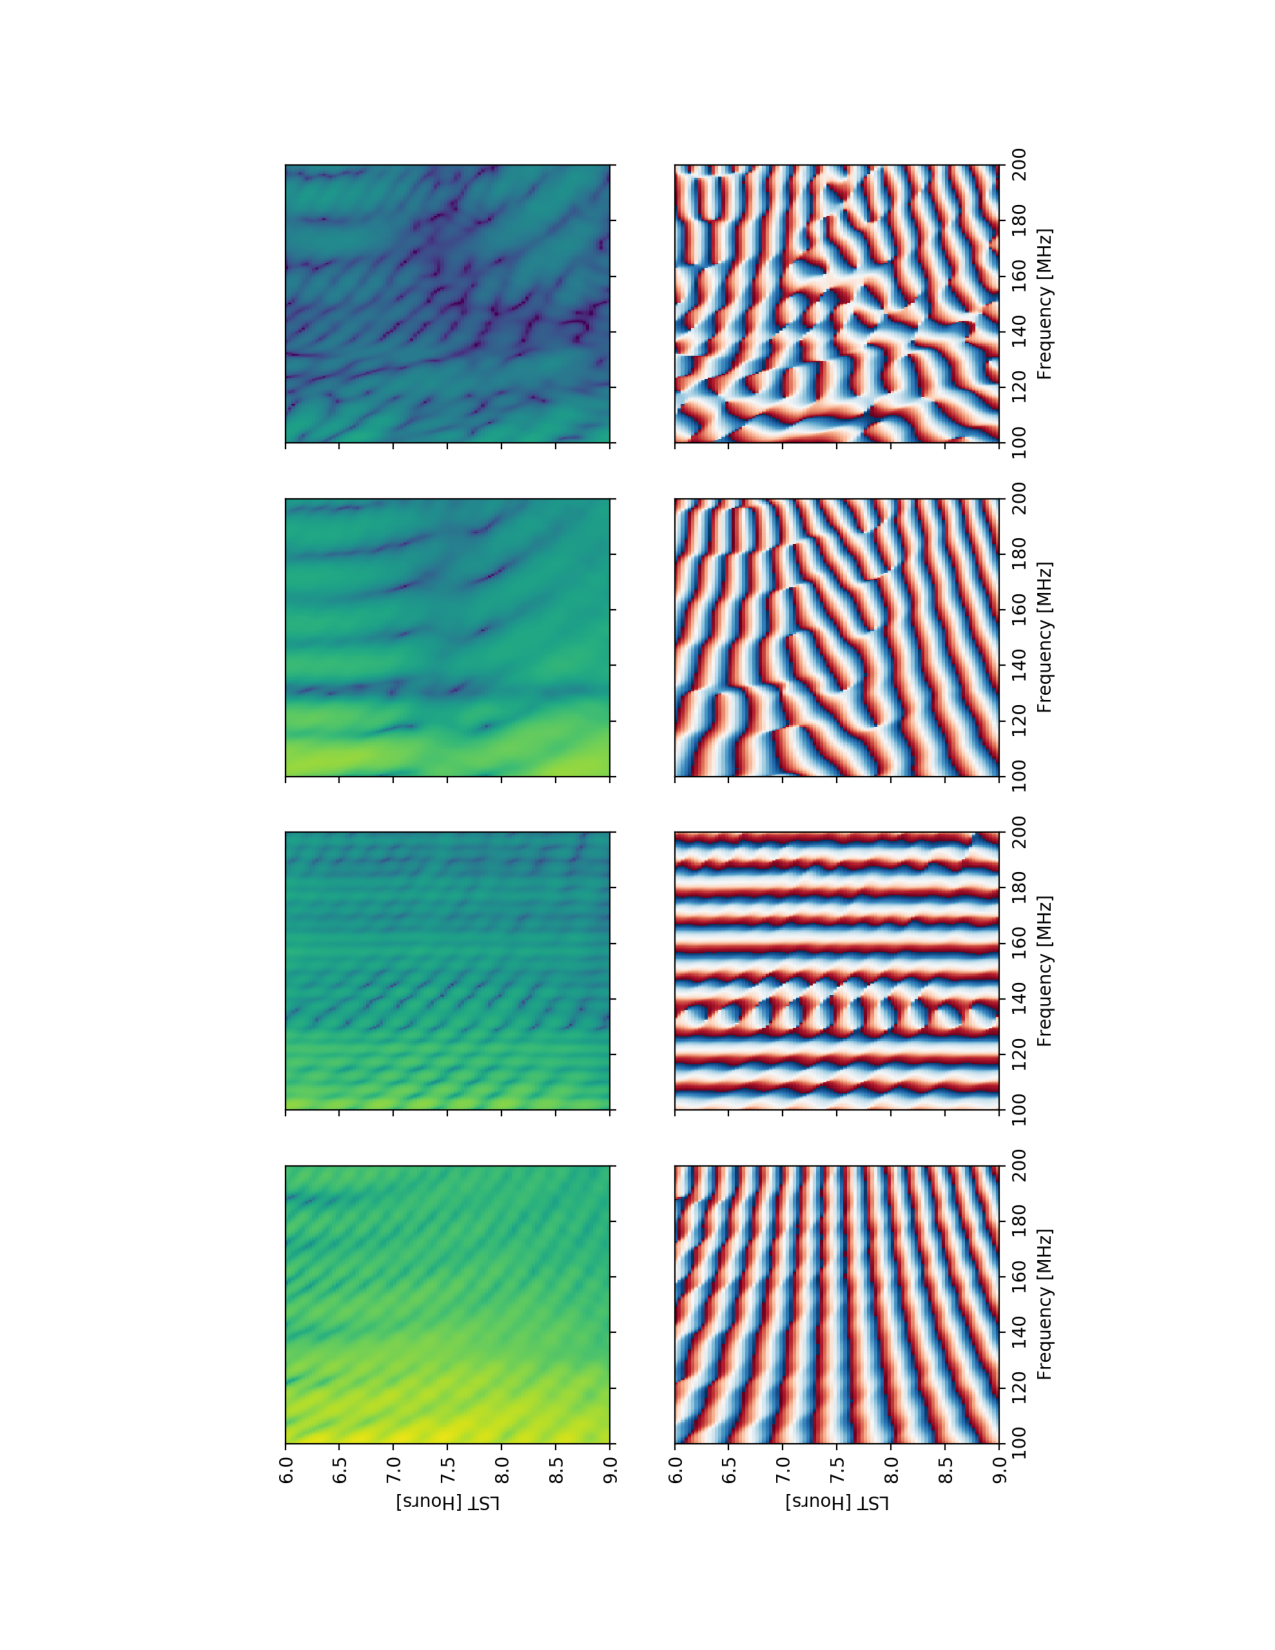
\includegraphics[width=0.6\textwidth, angle=270]{chapters/polcal/figures/sim_nonoise.pdf}
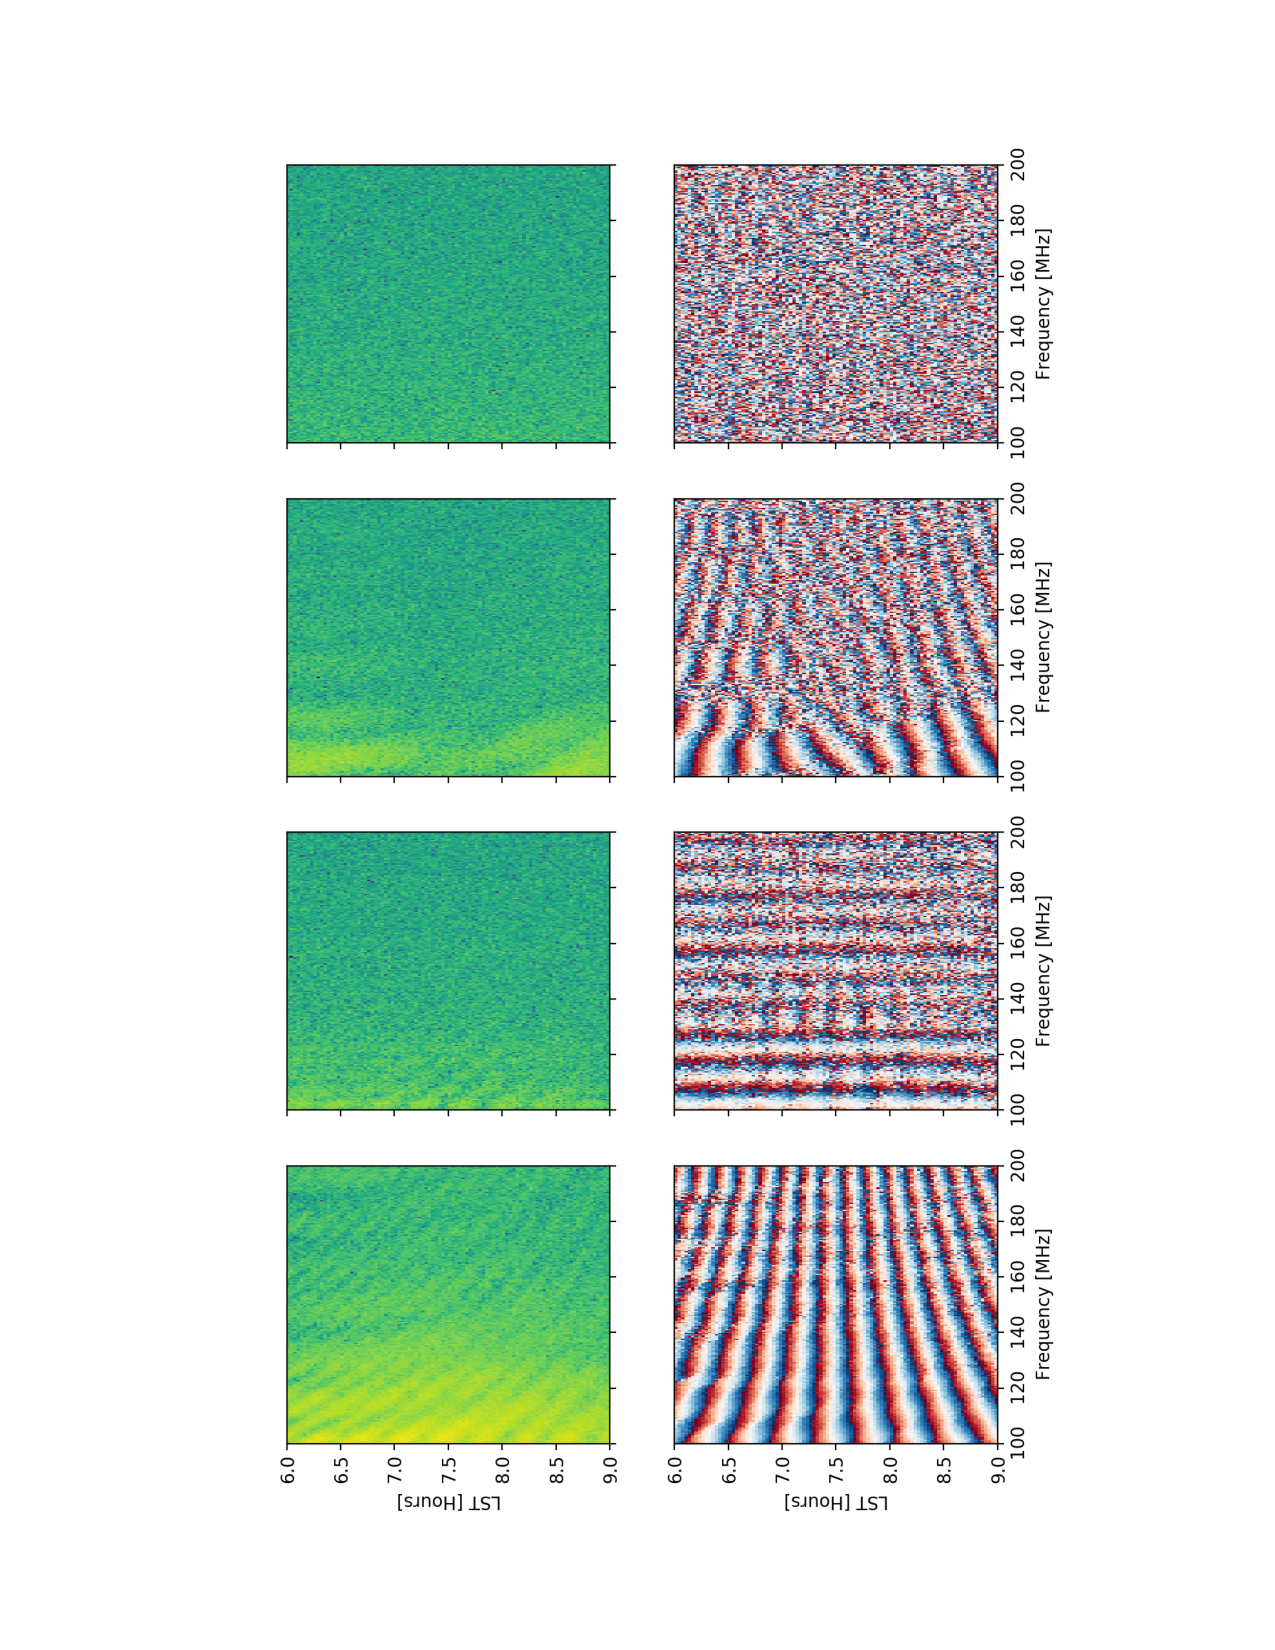
\includegraphics[width=0.6\textwidth, angle=270]{chapters/polcal/figures/sim.pdf}
\caption[Simulations of pseudo-Stokes visibilities,]{Simulations of absolute value (\textit{upper panels}) and phase (\textit{lower panels}) of pseudo-Stokes visibilities (left to right: pseudo-Stokes I, Q, U and V), as measured by a 30\,m East-West PAPER baseline. The upper group shows the noiseless simulation, and the lower shows the same simulation with the addition of a realistic PAPER noise model \citep{Moore.17}. Only a Stokes I sky was used -- all of the structure seen in $V_Q$, $V_U$ and $V_V$ can be attributed to direction-dependent leakage.}
\label{fig:simvis}
\end{figure}


\subsection{Data Processing}
\label{sec:polcal_data}

We tested these different calibration schemes on one night (JD 2456680.20 -- .65; January 22nd-23rd 2014; 6pm -- 6am South African Standard Time; Local Siderial Time 2 -- 13.5 hours) of PAPER 128-element observations. The PAPER-128 signal chain and full observation season results will be discussed in forthcoming publications, but we will provide a brief overview here. 

PAPER-128 consisted of 128 dual-polarization dipole receivers, 112 of which are arranged in a highly-redundant configuration, and the rest placed as in- and outriggers to the array in order to improve \textit{uv}-coverage; see Figure~\ref{fig:polcal_realarray}. Since all dipole arms were oriented North-South (`x') and East-West (`y'), \textit{xy} and \textit{yx} correlations have very low signal-to-noise compared to \textit{xx} and \textit{yy}.

All visibilities were RFI flagged using {\sc python} scripts from the {\sc aipy}\footnote{\url{https://github.com/HERA-Team/aipy}} library. These took the derivative of the frequency axis of all baselines associated with a given antenna and flagged any frequencies with a derivative 6$\sigma$ above the mean, per integration. We took the union of all baseline flags and applied them to the data. The 5\,MHz on both band-edges were always flagged. Compression proceeded as described in Appendix A of \cite{Parsons.14}, filtering to critical Nyquist sampling rates for the longest (300\,m) baseline of 493 kHz along the frequency axis (203 channels) and 42.9\,s along the time axis. 

\begin{figure}
\centering
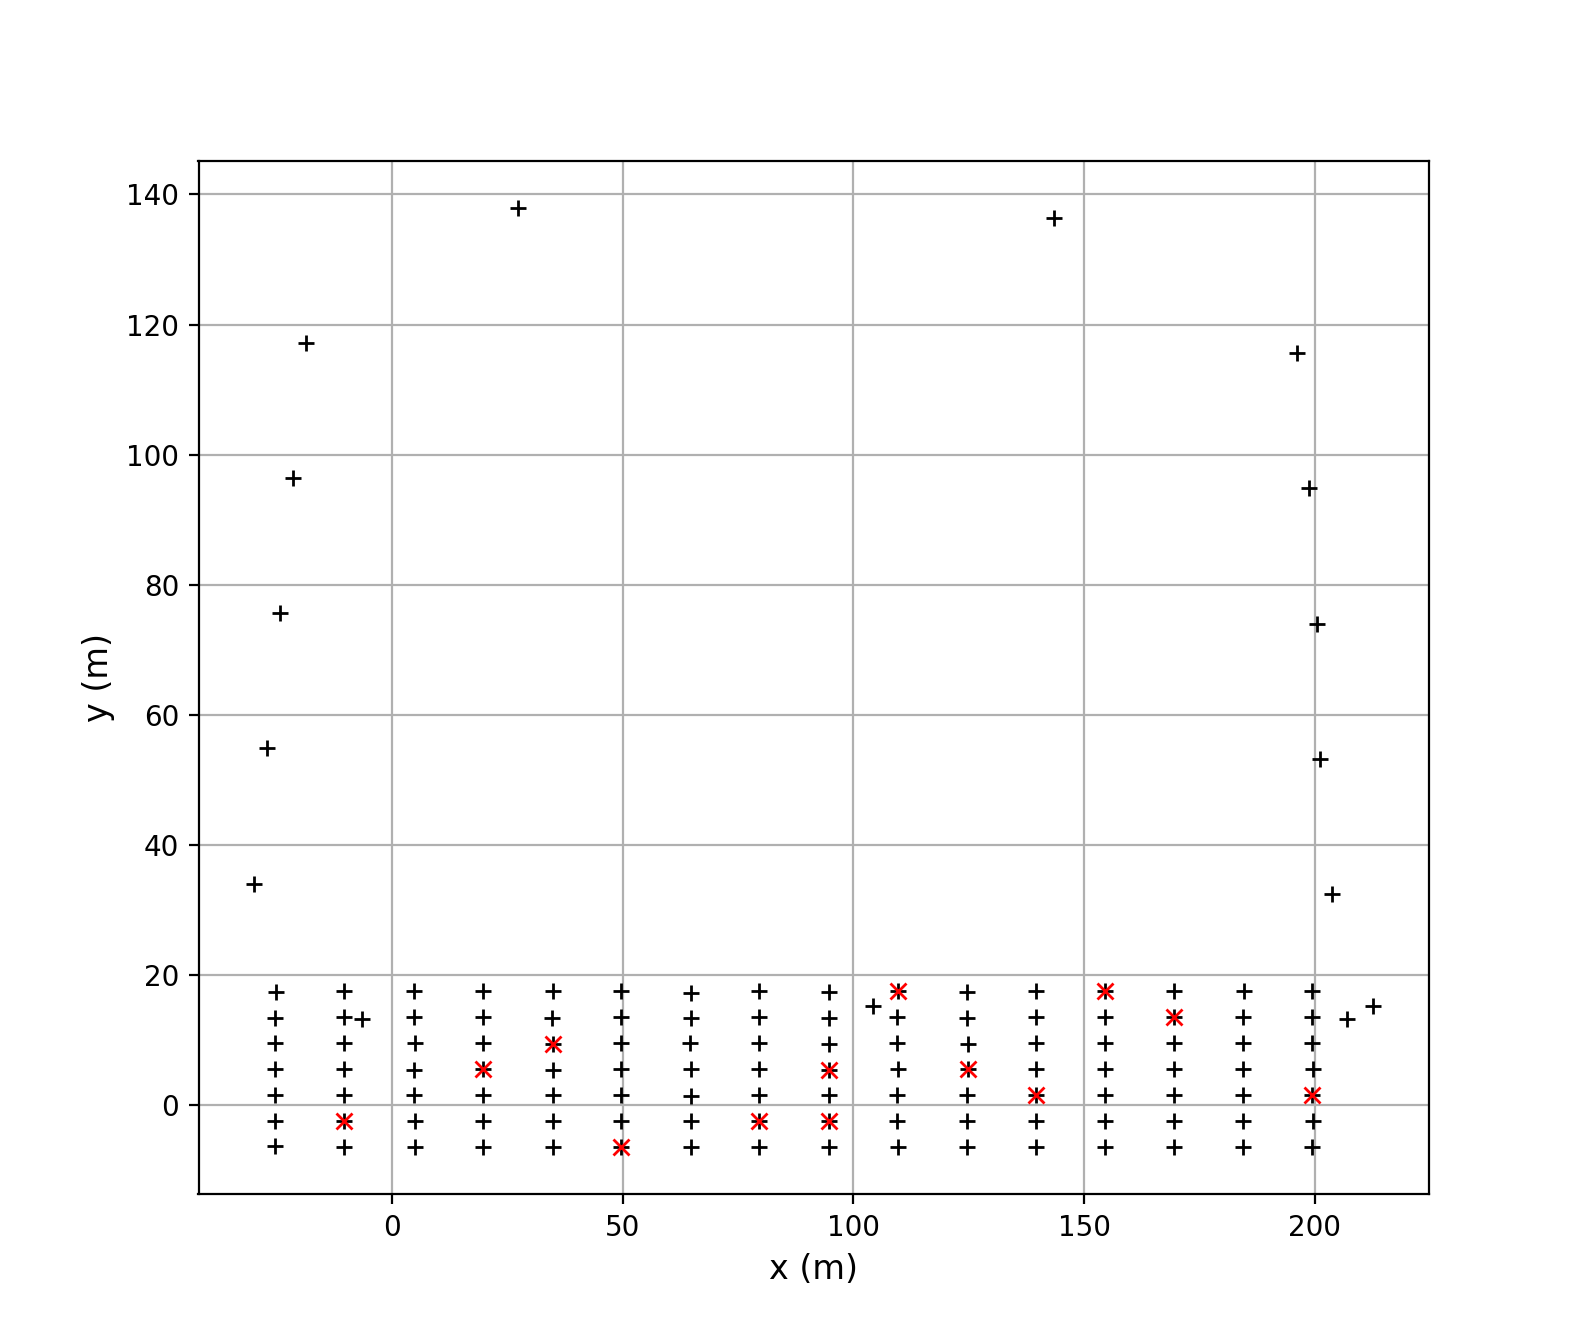
\includegraphics[scale=0.5]{chapters/polcal/figures/gridlayout.png}
\caption[Arrangement of the PAPER-128 array.]{Arrangement of the PAPER-128 array. Antennae determined to be malfunctioning are shown with red crosses and were excluded from analysis.}
\label{fig:polcal_realarray}
\end{figure}

After RFI flagging and compression, \textit{xx} and \textit{yy} visibilities were checked for erroneous behavior including 2$\sigma$ deviations from the median in number of RFI flags and mean visibility amplitude. Antennae exhibiting these behavior were excluded from further analysis (and are shown with red crosses in Figure~\ref{fig:polcal_realarray}). If an antenna qualified as `bad' in one polarization, it was excluded in all of them. Also note that we could only calibrate the 112 antennae in the redundant grid using {\sc omnical}.

For the least-squares fit to converge at the \textit{logcal} stage of calibration, visibilities cannot exhibit phase-wraps, since the system of equations solved at this stage are insensitive to additive offsets of $2\pi$ in their imaginary parts (\textit{lincal} will be able to re-insert these as required; \citealt{Liu.10}). Therefore we had to flatten the phases on all visibilities prior to any implementation of {\sc omnical}. We were able to do this redundantly without reference to the sky; taking the ratio of redundant (uncalibrated) visibilities together and averaging over time, defined as:

\begin{equation}
\mathcal{V}(\nu) = \langle V_{ij, pq}(\nu,t)V^*_{kl, pq}(\nu,t) \rangle_t .
\label{eq:Vijratio}
\end{equation}

Because this is the ratio of two nominally-redundant visibilities (i.e. baselines $ij$ and $kl$ belong to the same redundant group with model visibility $V_{|i-j|,pq}$), and the measurements are not yet calibrated, we can expand Equation~\ref{eq:Vijratio} as

\begin{equation}
\mathcal{V}(\nu) = \langle g^*_{p,i}g_{q,j}g_{p,k}g^*_{q,l} |V_{|i-j|,pq}|^2 \rangle_t .
\end{equation}
Writing the complex gains as $g_{p,a}=G_{p,a} e^{-i\nu\tau_{p,a}}$ for antenna $a$, we can reduce the product of gain-amplitudes and the squared visibility into some frequency-dependent function, and an exponential product of gain phase terms

\begin{equation}
\mathcal{V}(\nu) = K(\nu)\exp\left(i\nu (\tau_i - \tau_j - \tau_k + \tau_l)\right) .
\end{equation}
A Fourier transform along the frequency axis (which we term a \textit{delay transform}; \citealt{Parsons.12a}) of $\mathcal{V}(\nu)$ gave a function that was sharply-peaked at a given delay

\begin{equation}
\tilde{\mathcal{V}}(\tau) = \tilde{K}(\tau)*\delta_D\left(\nu (\tau_i - \tau_j - \tau_k + \tau_l)\right).
\end{equation}
We can define a variable as the maximum of the above function:

\begin{equation}
\mathcal{T}_{ijkl}(\tau) = {\tt max} | \tilde{\mathcal{V}}(\tau) |,
\end{equation}
which will occur at value 

\begin{equation}
\tau = \tau_{\rm max} = \nu (\tau_i - \tau_j - \tau_k + \tau_l).
\end{equation}
With enough redundant baselines involving antennae $i,j,k$ \& $l$ this is a linearly-solvable set of equations for each value of $\tau$. Multiplying $V_{ij}$ by $e^{-2\pi i \nu (\tau_i - \tau_j)}$ by definition flattened the phase across the band. This method was very sensitive to signal-to-noise, so these initial phase estimates were created with $p=q$; that is \textit{xx} and \textit{yy} visibilities only. The estimates were then applied to all visibilities appropriately. We could then run {\sc omnical} according to each of the schemes described in Section~\ref{subsec:calSchemes}.

\subsection{Results}
\label{sec:polcal_results}

We ran {\sc omnical} using the \textit{2pol}, \textit{4pol} and \textit{4pol+minV} schemes, which granted complex gain values for each antenna feed in the redundant grid. In this Section we chose to concentrate our analysis on the 30\,m East-West spacings used for PAPER power spectrum studies.

\subsubsection{Calibration}

The complex-gains dataset alone was highly multidimensional. We chose to analyze short time- and frequency- averages for these data. For example, the $\langle | g^{\rm 2pol}_{x,a} | \rangle_{t,\nu}$ notation indicates the average of the absolute value of the gain value for antenna $a$, polarization `x' in the \textit{2pol} calibration scheme. The average was over 10 minutes (the length of a single {\sc miriad} file produced by the PAPER correlator) and a 10\,MHz band running from 145 to 155 MHz (the center of the PAPER band, generally clear of RFI and used for power spectrum analyses).

Figure~\ref{fig:4pol-geo-angle} shows $\langle {\rm arg}( g^{\rm 2pol}_{a} ) \rangle_{t,\nu}$, the average phase of the gain calibration for `x' and `y' polarizations. It very clearly shows the phase-slope degeneracy present for both dipole orientations, sloping in opposite directions. 

\begin{figure}
\centering
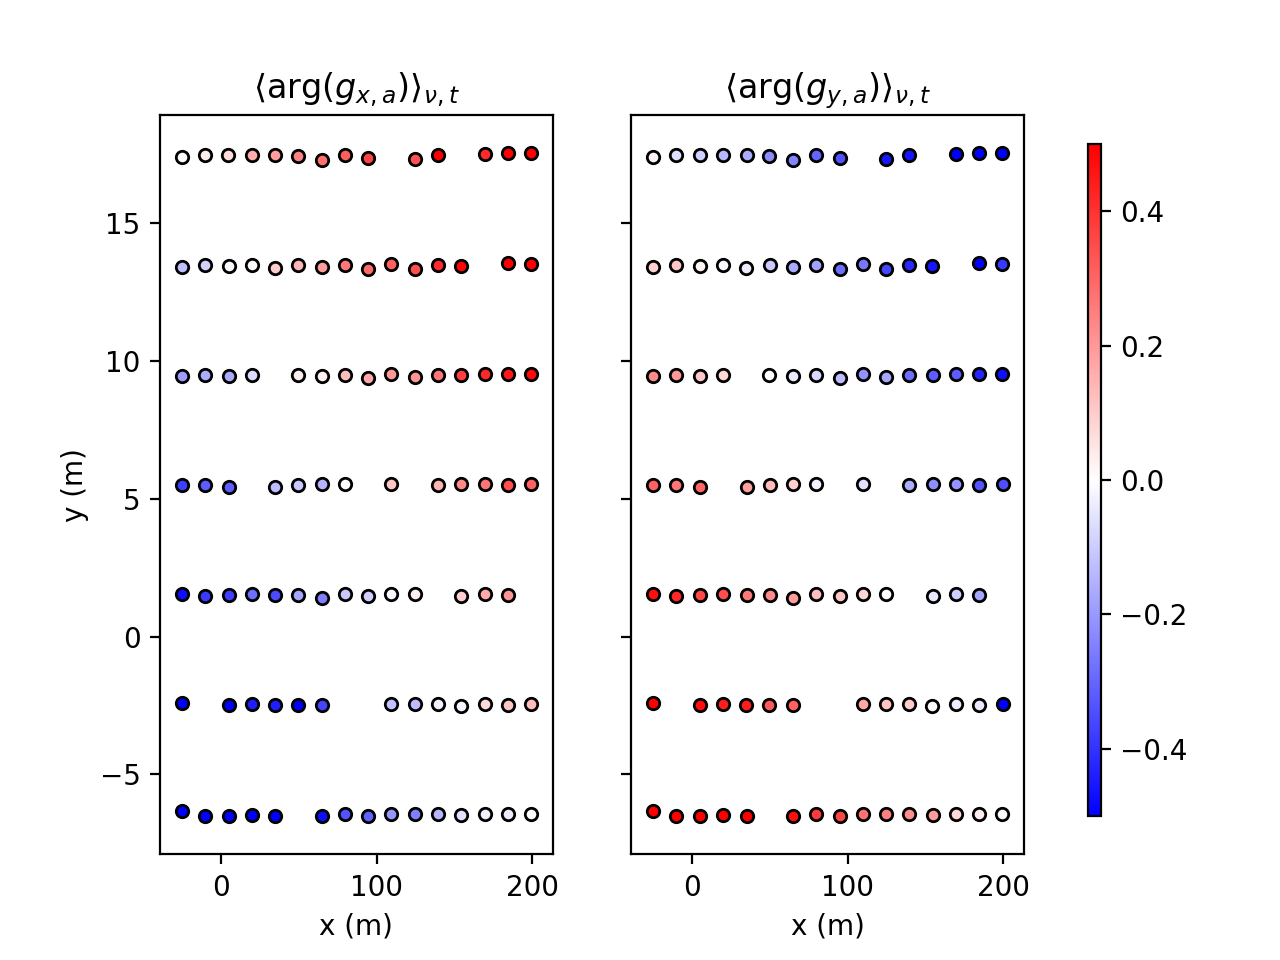
\includegraphics[scale=0.5]{chapters/polcal/figures/4pol_geo.png}
\caption[The phase of the complex gain value for the \textit{4pol} calibration scheme.]{The phase of the complex gain value for the \textit{4pol} calibration scheme is shown on the color axis (radians) for the redundant grid. The phase of the `x' gains is shown on the left, and the `y' gains on the right. The phase-slope degeneracy is clear in both panels, as is the fact that the slope is in opposite directions for the two dipole orientations.}
\label{fig:4pol-geo-angle}
\end{figure}

Figure~\ref{fig:diff-gains} shows the differences in `x' gain solutions between calibration schemes. 
The difference between \textit{4pol} and \textit{4pol+minV} was consistently smaller than the difference of either of these with the \textit{2pol} scheme. 

As noted in Section~\ref{subsubsec:degen}, {\sc omnical} tried to fix the average gain amplitude over the array to unity to avoid drifts in the amplitude degeneracy from sample to sample, so we were able compare amplitude calibrations in terms of percentage deviation. The average difference in gain amplitude per antenna between \textit{2pol} and \textit{4pol} was 3.5\%, between \textit{2pol} and \textit{4pol+minV} was 2.9\%, and was 0.7\% between \textit{4pol} and \textit{4pol+minV}. The $\sim$30 degree spread in the differenced phases between the \textit{2pol} scheme and the other two was likely due to different realizations of phase degeneracies between these calibration schemes.

\begin{figure}
\centering
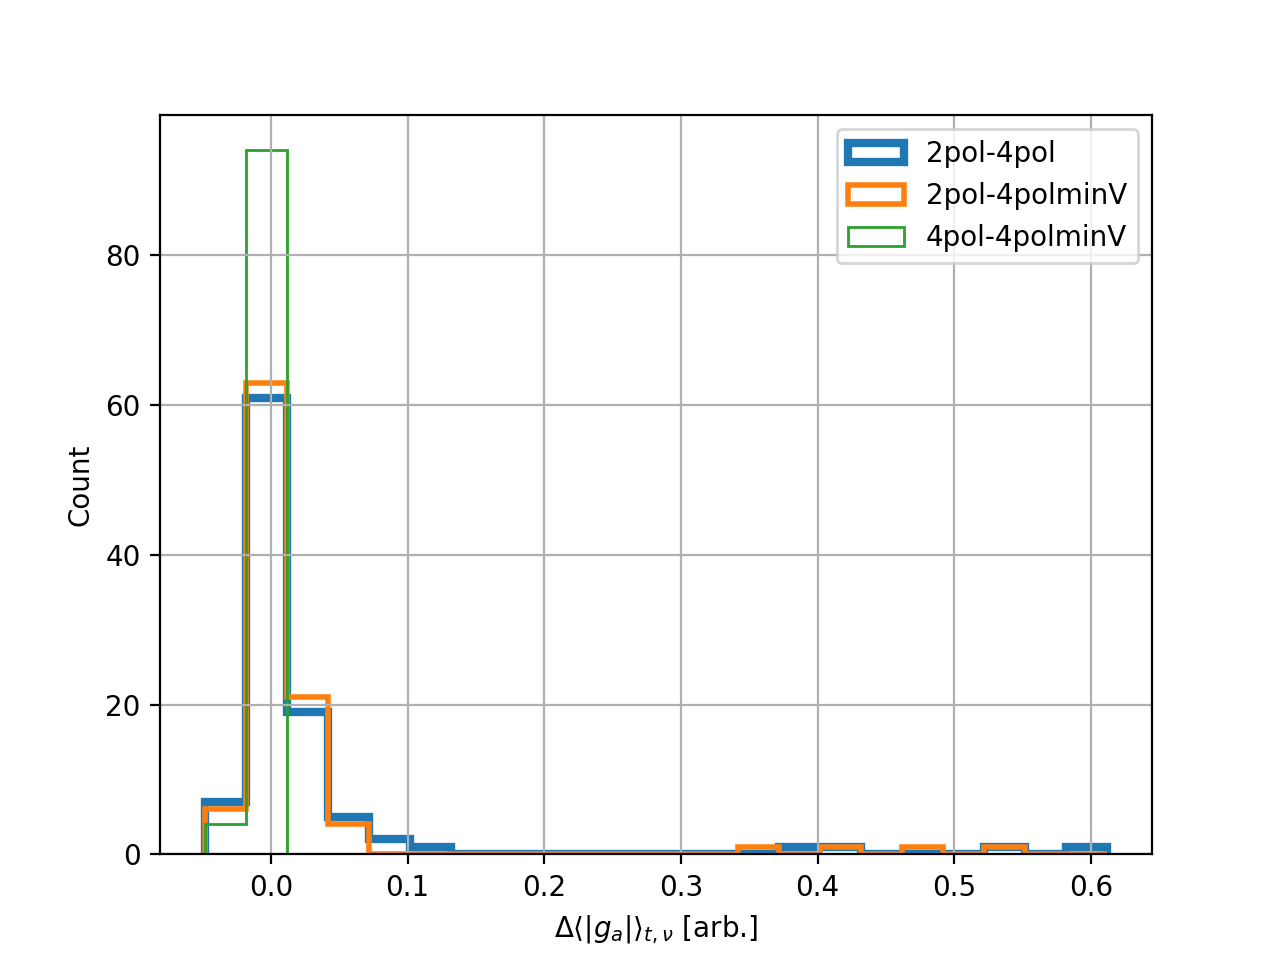
\includegraphics[scale=0.5]{chapters/polcal/figures/dGainHist.png}
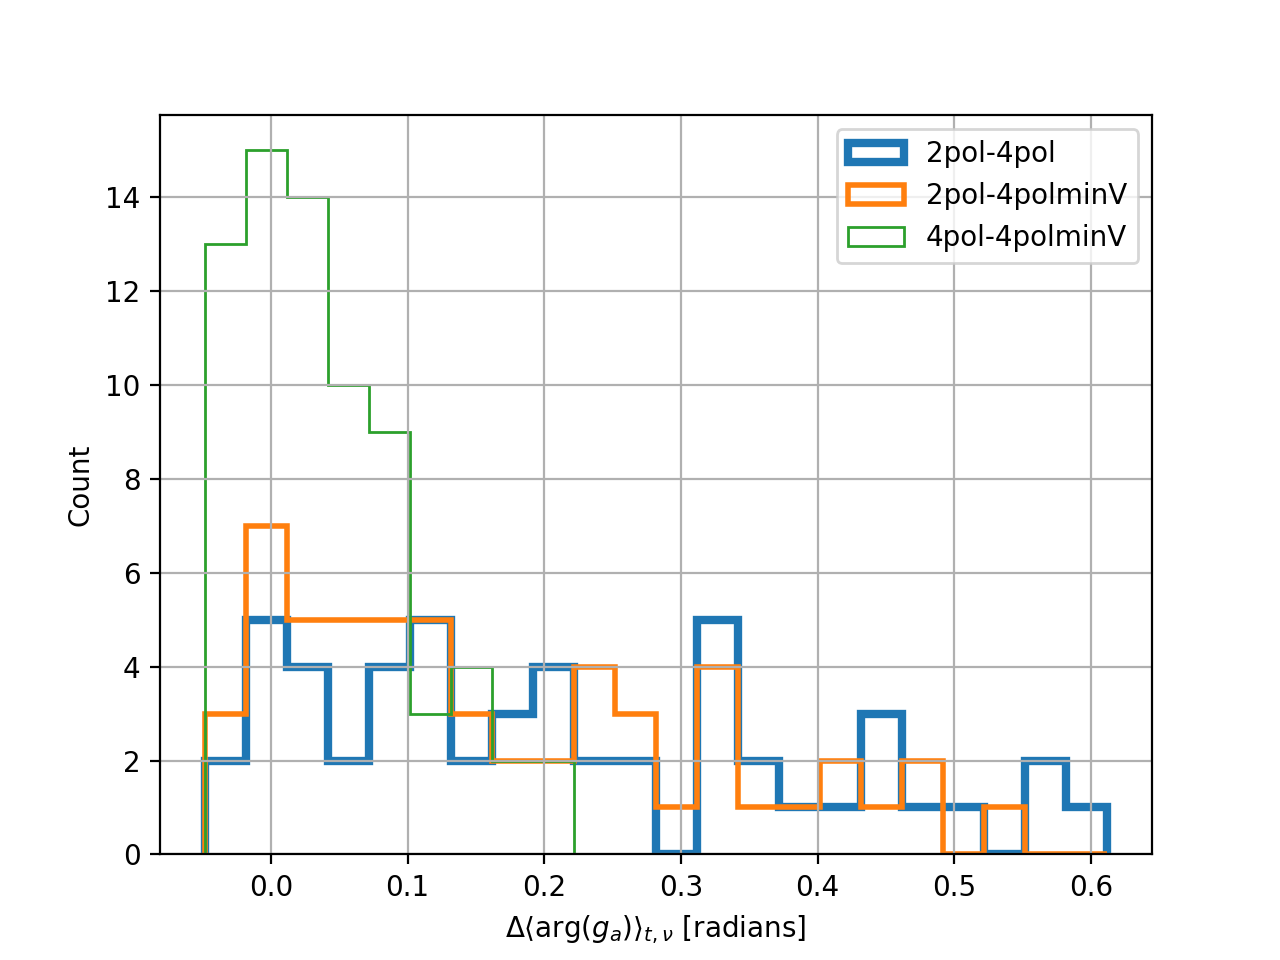
\includegraphics[scale=0.5]{chapters/polcal/figures/dAngleHist.png}
\caption[Histograms of differences in the `x' gain calibrations per antenna between calibration schemes.]{Histograms of differences in the `x' gain calibrations per antenna between calibration schemes. Above: difference in absolute value. Below: difference in phase.
For most antennae, absolute value of the gain does not change by large amounts between calibration schemes; most of the change takes place in the phase.
The difference between \textit{4pol} and \textit{4pol+minV} is consistently smaller than the difference of either of these with the \textit{2pol} scheme. This is likely a sign of different realizations of phase degeneracies between calibration schemes.}
\label{fig:diff-gains}
\end{figure}


Figure~\ref{fig:polcal_chisq} shows the sum of $w^2$ values (see Equation~\ref{eq:polcal_w2}) over all antennas in the array for each feed polarization in each of the three calibration schemes. The color scale is logarithmic. Clearly, the \textit{2pol} scheme achieves a much greater level of redundancy in each feed polarization throughout the band. Towards the end of the night, the Galaxy was in the far side-lobes of the PAPER beam and introduces higher sky temperatures, which accounted for the trend in all calibration schemes performing worse towards the end of the night. However, the reason for rapid transitions in $w^2$ at Local Sidereal Time $\sim 10.5$ in the \textit{4pol} and \textit{4pol+minV} schemes is not well understood. In general, $w^2$ was an order of magnitude higher for the \textit{4pol} and \textit{4pol+minV} schemes.

\begin{figure}
\centering
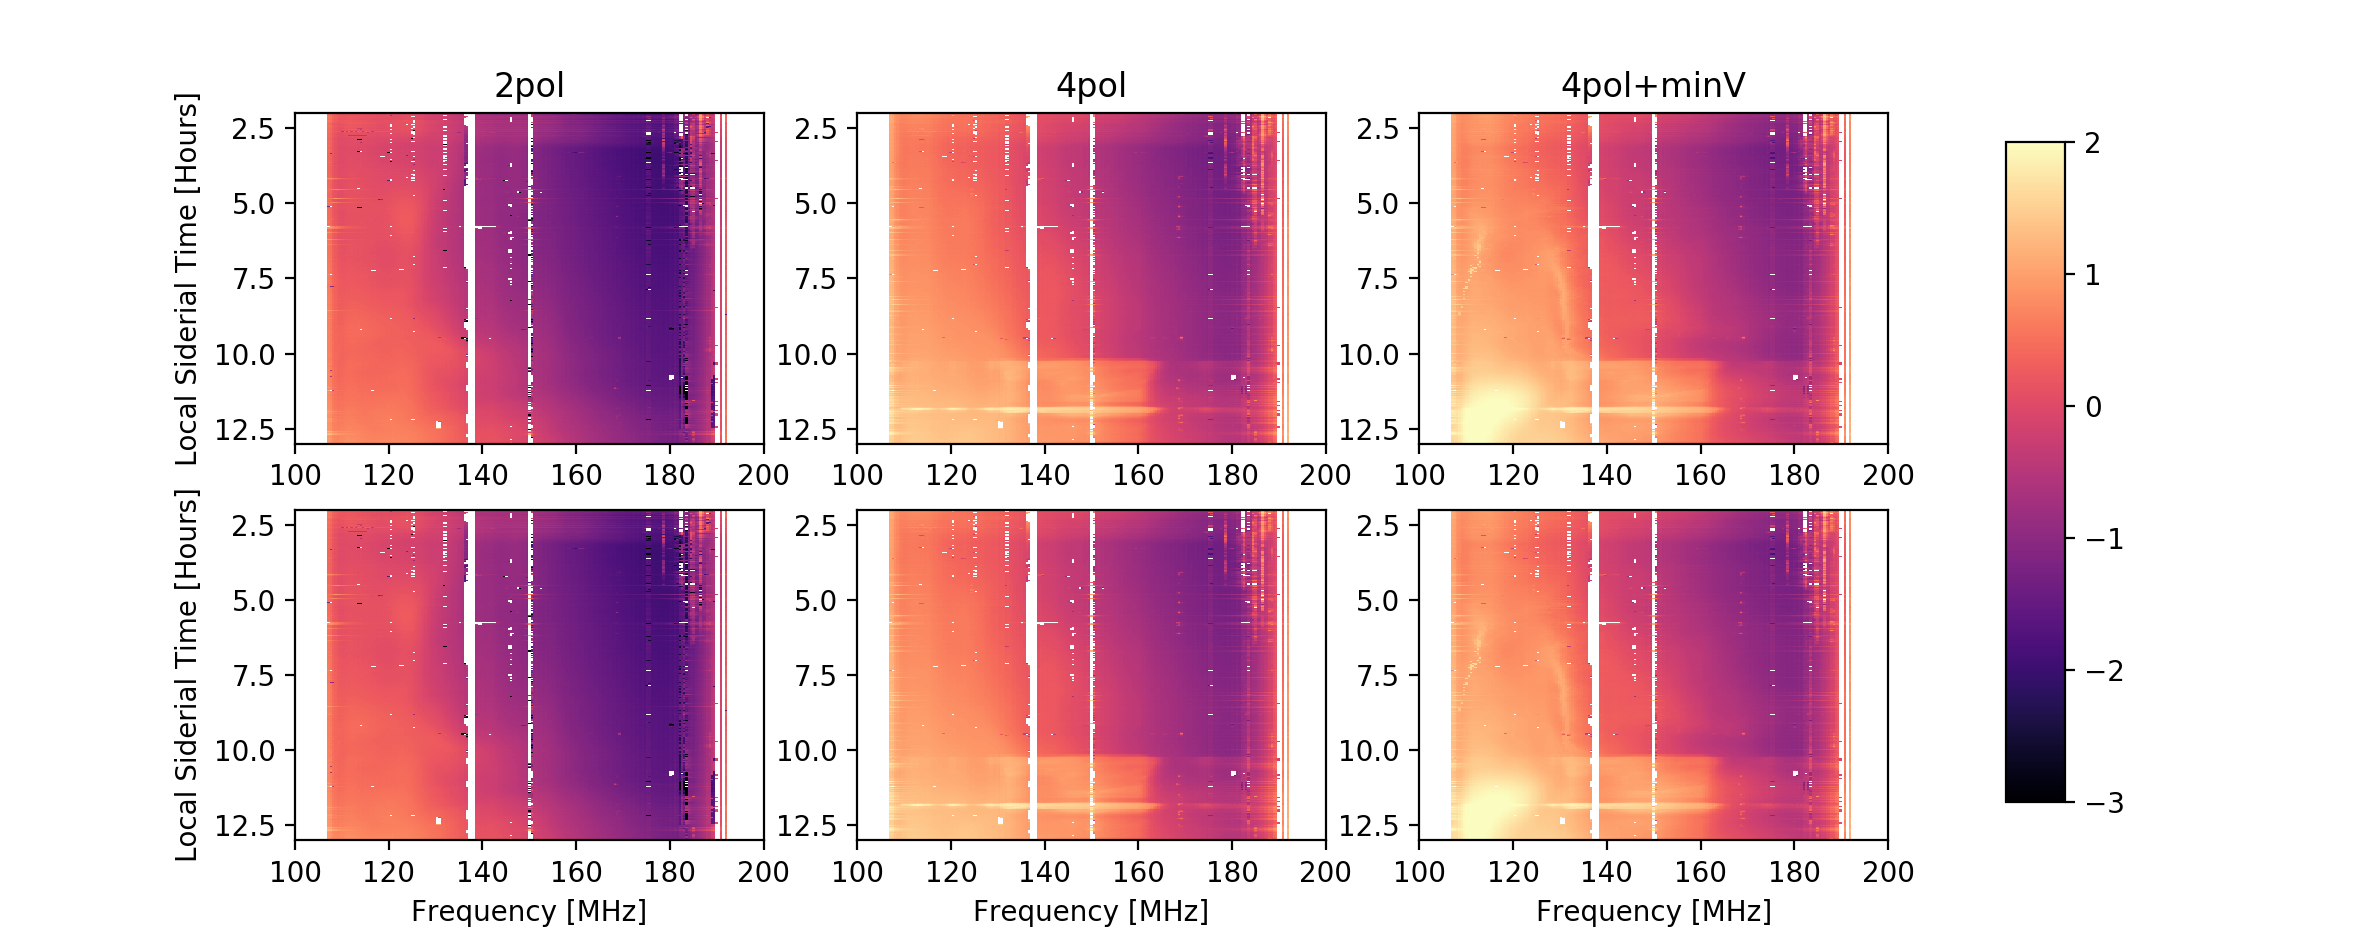
\includegraphics[width=0.75\textwidth]{chapters/polcal/figures/chisq.png}
\caption[$w^2$ values, summed across the array.]{$w^2$ values, summed across the array, for the $x$ (above) and $y$ (below) feeds in different calibration schemes. From left to right: \textit{2pol}, \textit{4pol} and \textit{4pol+minV}. The color axis is logarithmic, in arbitrary data units. The white gaps are due to RFI flagging.}
\label{fig:polcal_chisq}
\end{figure}

\subsubsection{Pseudo-Stokes Visibilities}

Applying the complex gains to the visibilities, we constructed pseudo-Stokes visibilities. These data are shown in Figure~\ref{fig:pseudo-stokes-grid}. Figure~\ref{fig:delay-stokes-grid} shows the delay-transformed pseudo-Stokes visibilities. The ``stripe" of power across the frequency axis within the first 100 integrations was a thermal effect due to the sun not yet being fully below the horizon.

\begin{figure}
\centering
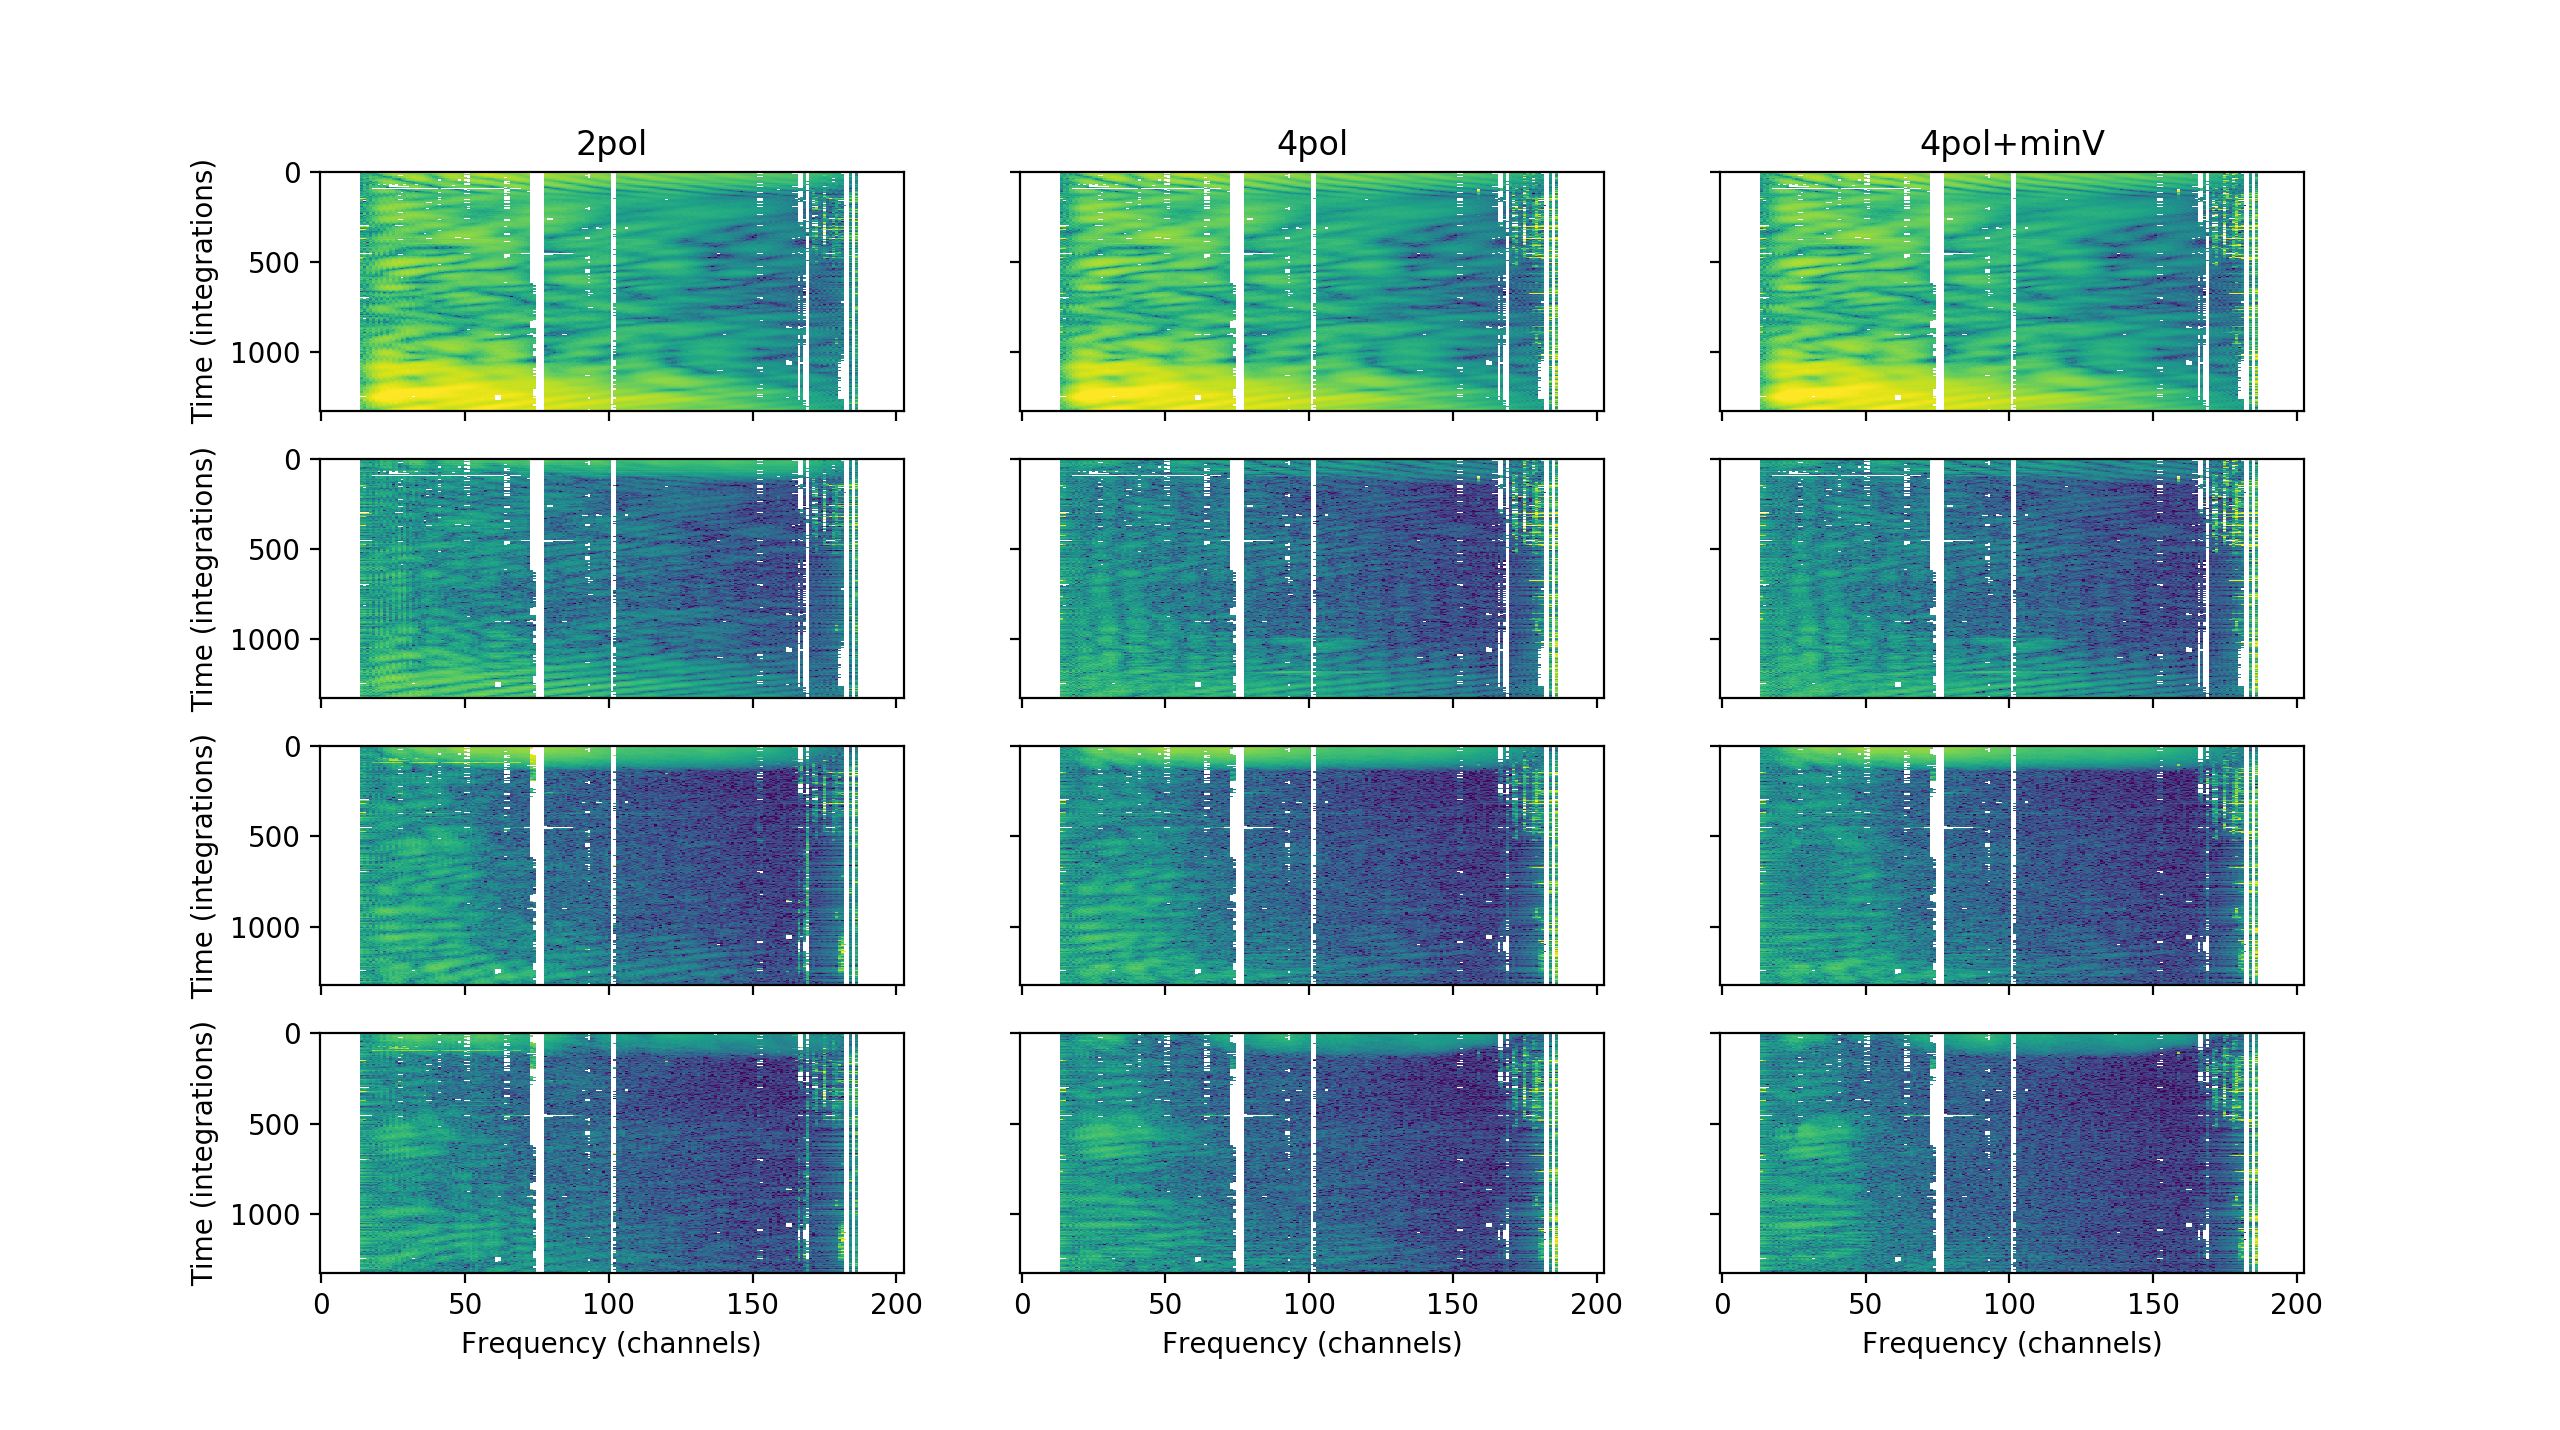
\includegraphics[scale=0.5]{chapters/polcal/figures/vis.png}
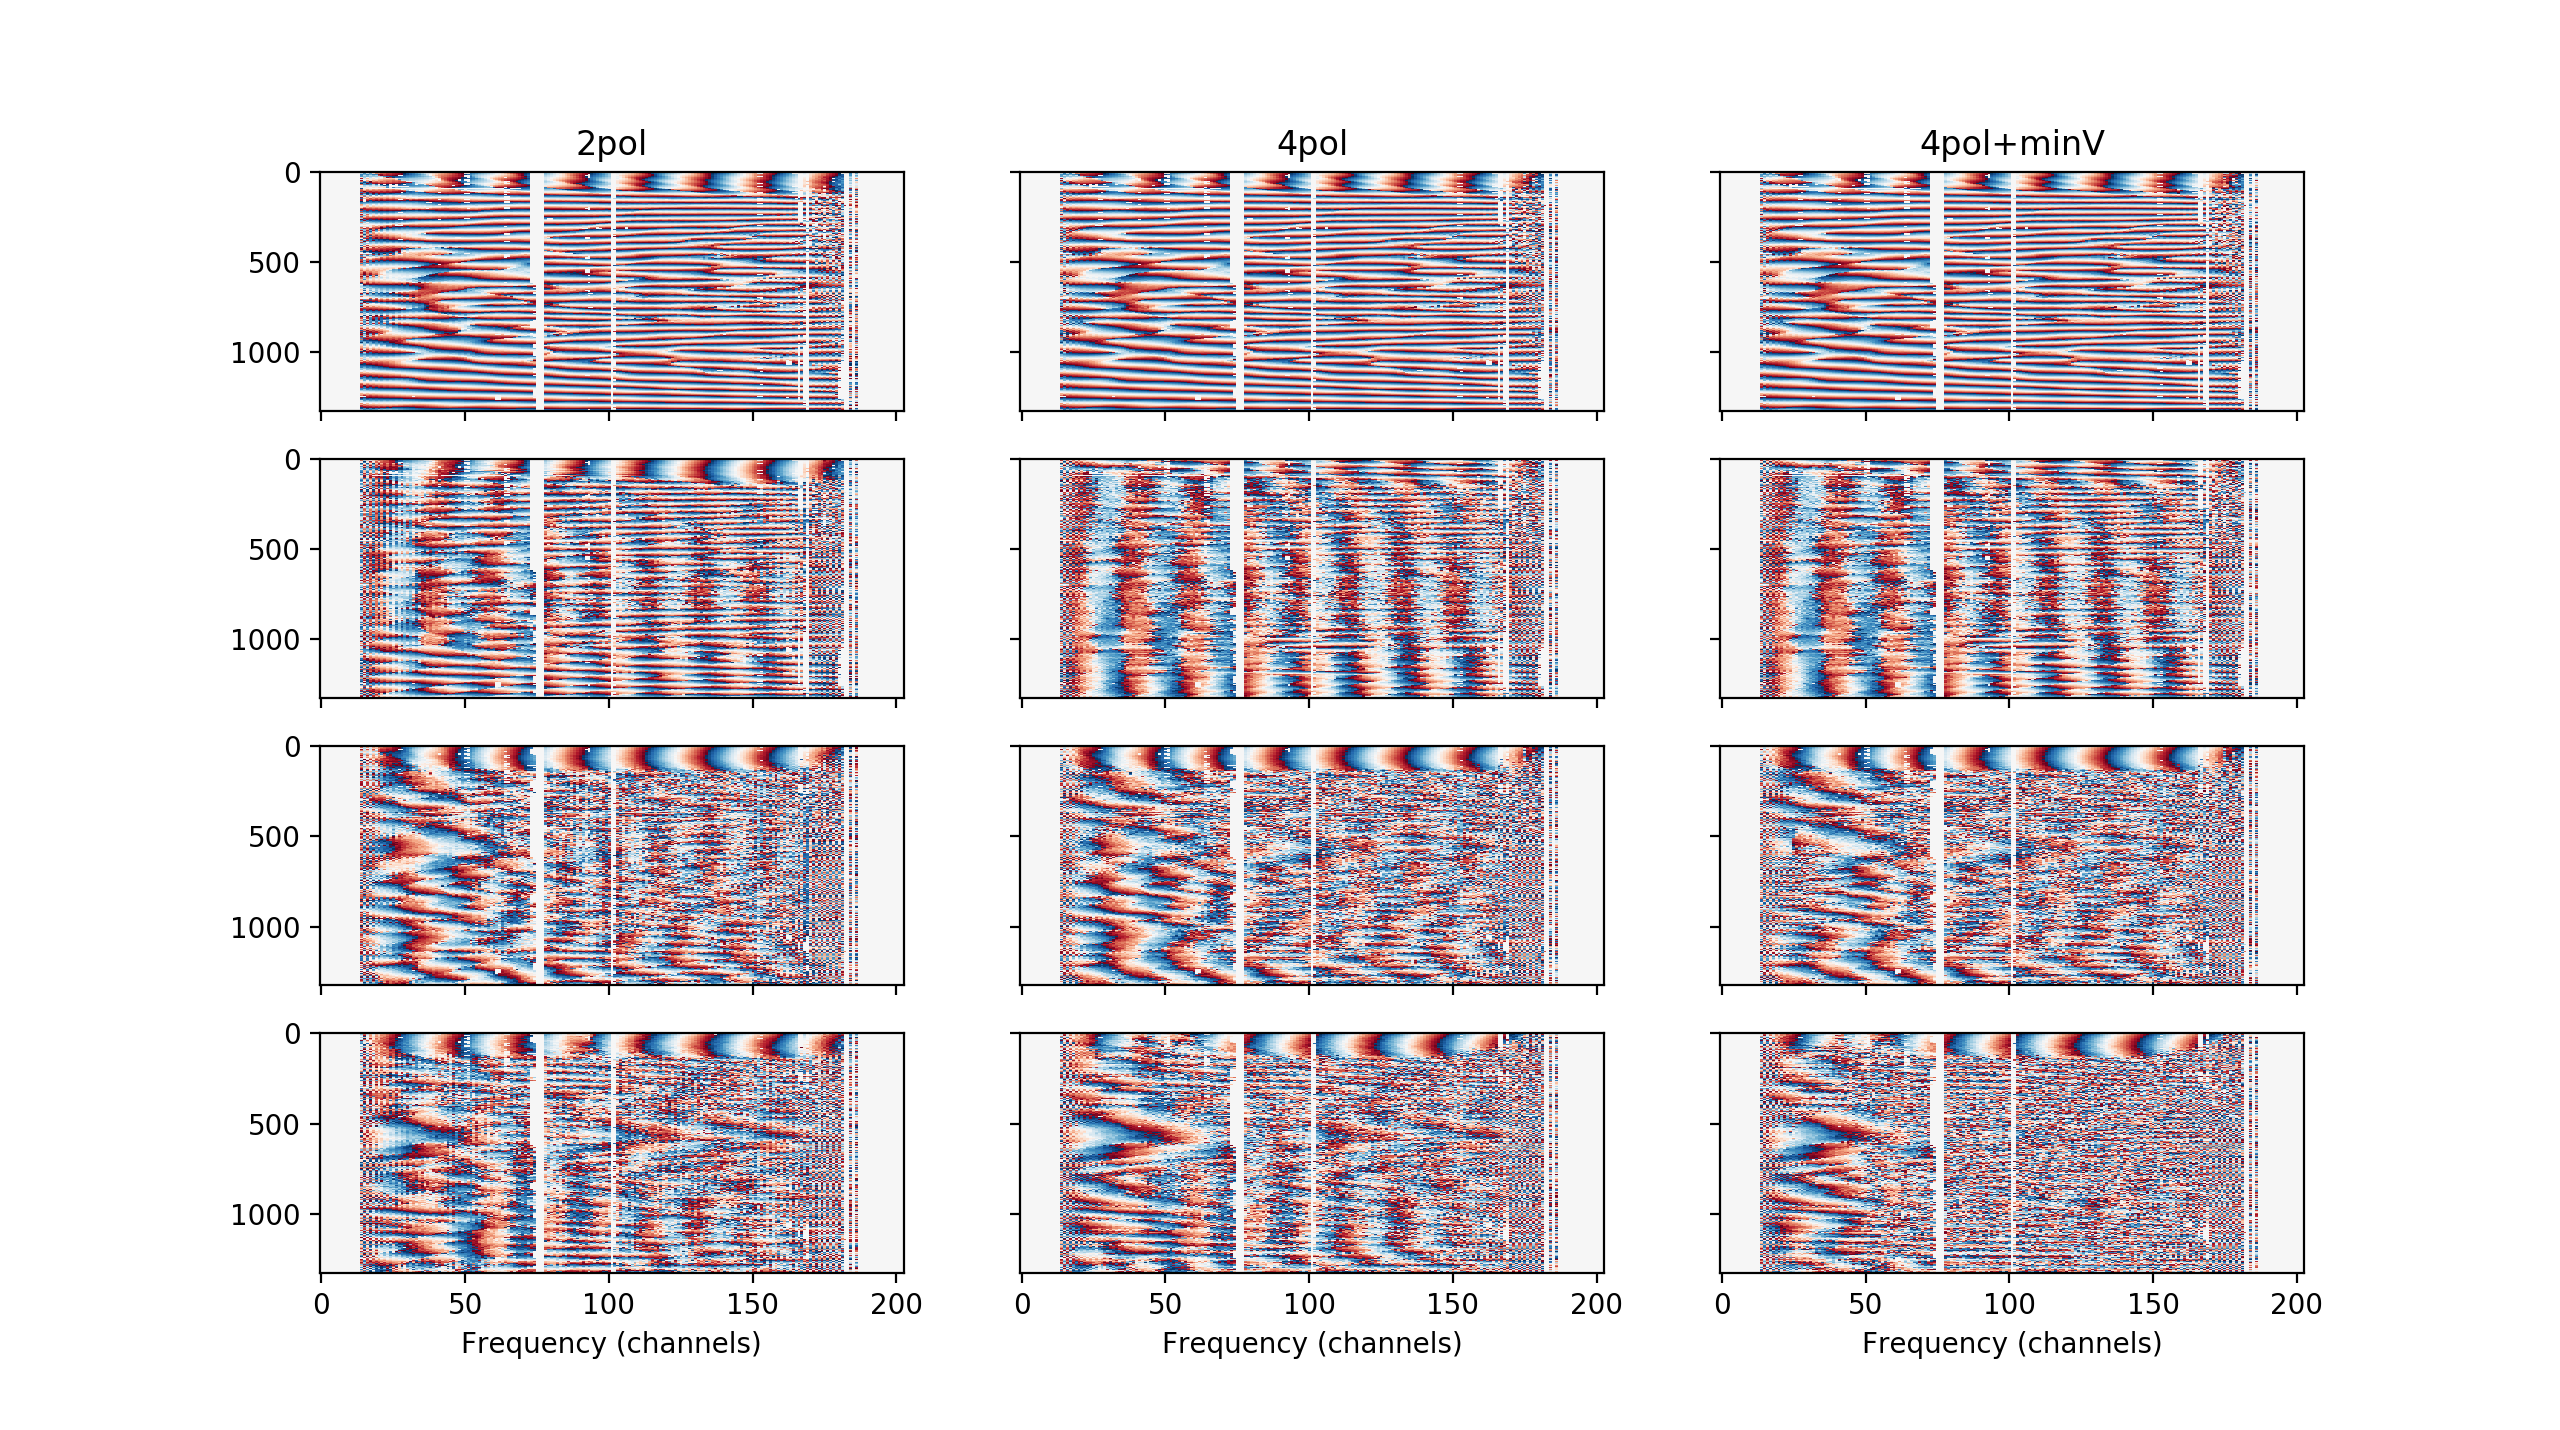
\includegraphics[scale=0.5]{chapters/polcal/figures/phase.png}
\caption[Pseudo-Stokes visibility amplitudes and phases.]{Pseudo-Stokes visibility amplitudes (\textit{top}) and phases (\textit{bottom}). Amplitudes are plotted on a logarithmic color scale that spans 3 orders of magnitude (without absolute calibration, this scale is in arbitrary units). Phases are on a linear scale of $-\pi$ to $\pi$. The three columns correspond to the three different calibration schemes. Rows are from top to bottom: $V_I$, $V_Q$, $V_U$, and $V_V$.}
\label{fig:pseudo-stokes-grid}
\end{figure}

The upper panels in Figure~\ref{fig:pseudo-stokes-grid} -- the absolute-valued visibilities -- show that Stokes I power was dominant given any calibration scheme used. This was expected, since the linear polarizations had much higher signal-to-noise than the cross polarizations that form $V_U$ and $V_V$. We saw that the amplitude of pseudo-Stokes Q was reduced across the band in the \textit{4pol} and \textit{4pol+minV} schemes. This was  also expected, given that these calibration schemes allowed information in $xx$-polarized visibilities to influence the calibration of $yy$-polarized ones, and vice-versa. In the regime of a single night's observation, we did not expect to observe substantial power from the Stokes Q sky \citep{Kohn.16, Lenc.16, Moore.17}. Although we set no specification on the Stokes Q sky during calibration, we observe our gain solutions tending towards lower Stokes Q power during polarized redundant calibration. 

A similar but less-substantial difference was seen in the pseudo-Stokes U visibility amplitudes, but an interesting interplay between pseudo-Stokes U and V was more clearly seen in the delay-transformed visibilities in Figure~\ref{fig:delay-stokes-grid}. First, we must observe that the \textit{4pol+minV} calibration scheme worked as expected, reducing the amplitude of pseudo-Stokes V across most of the band. In Figure~\ref{fig:delay-stokes-grid}, we show that the difference between the foreground signal for pseudo-Stokes U and V in the \textit{4pol} case, compared to the \textit{4pol+minV} case, was the increase in U signal and the decrease of V. This effect was observed in \cite{Kohn.16} when minimizing pseudo-Stokes V using an array-wide constant, as opposed to the per-sample basis implemented in this work. It is mathematically consistent with partially accounting for uncalibrated \textit{D}-terms on each feed.

We also note that the lowest frequencies in the band (below channel 70) are consistently poorly behaved. This is a property seen in many PAPER measurements \citep[e.g.][]{Jacobs.15, Moore.17} and is due to brighter foregrounds at low-frequencies, a larger solid angle of the beam, and higher receiver temperatures at lower frequencies.

\begin{figure}
\centering
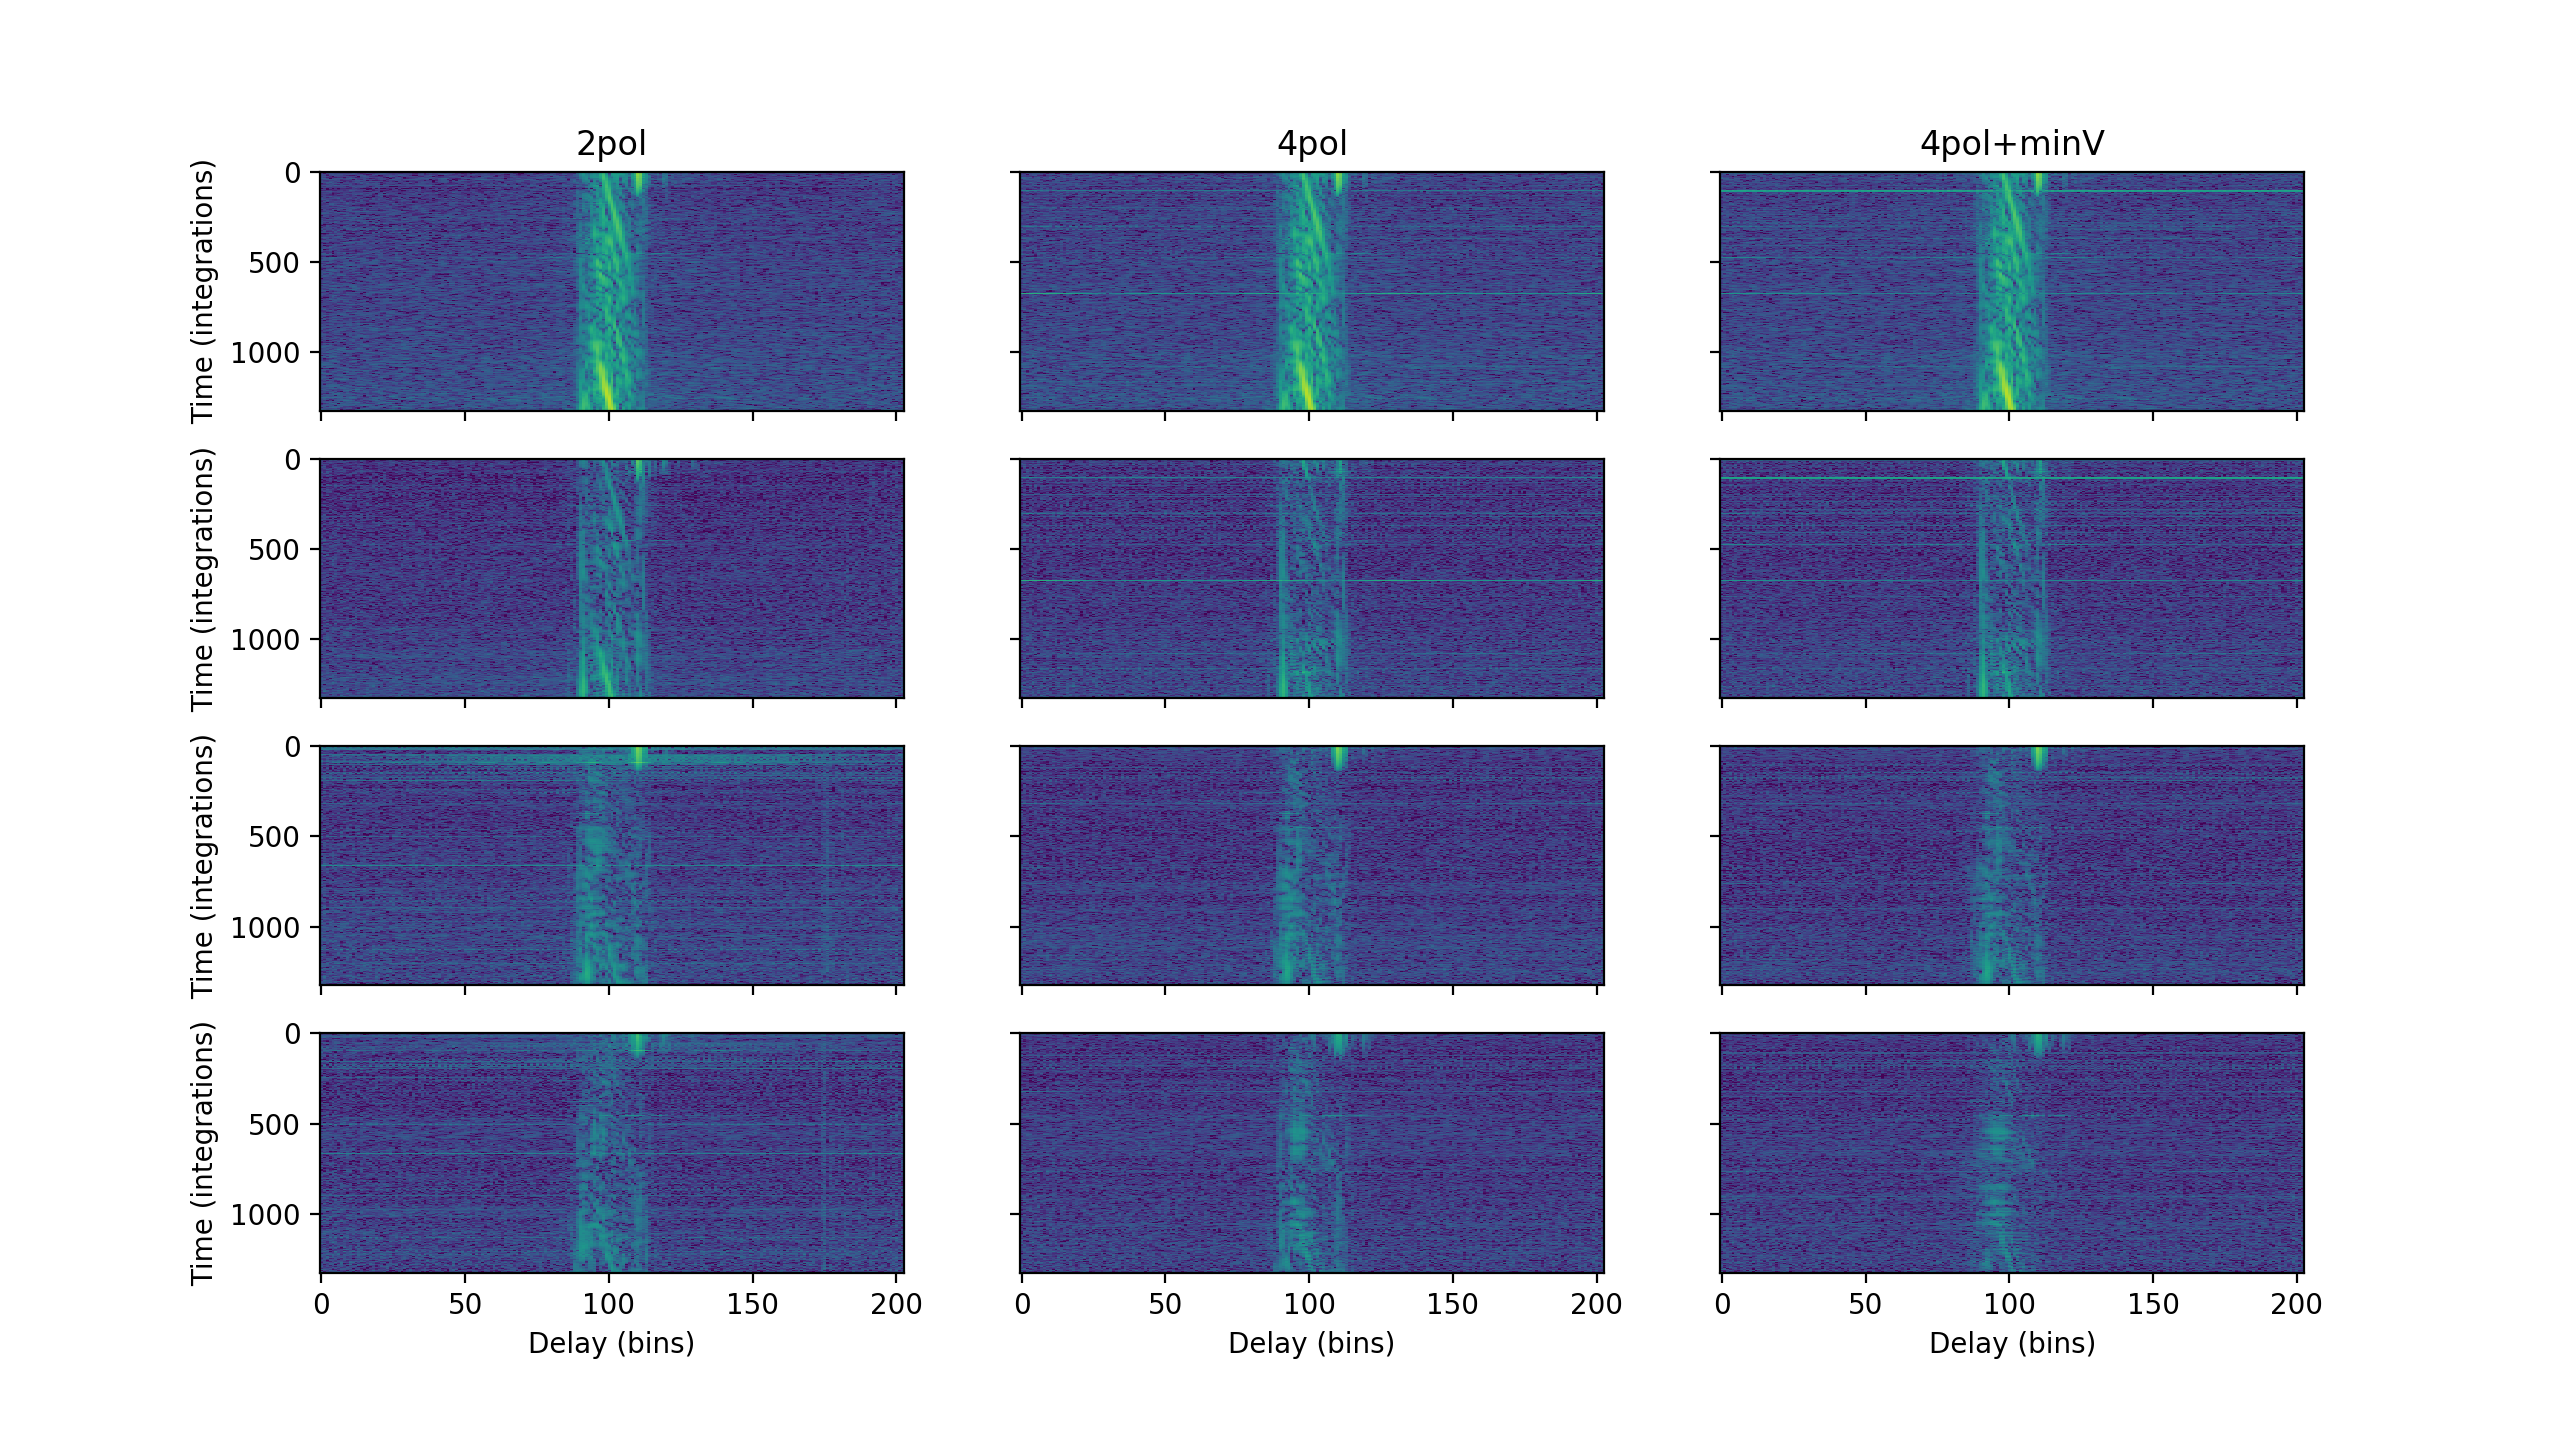
\includegraphics[scale=0.5]{chapters/polcal/figures/dly.png}
\caption[Delay-transformed pseudo-Stokes visibilities.]{Delay-transformed pseudo-Stokes visibilities. Plotted on a logarithmic color scale that spans 4 orders of magnitude (without absolute calibration, this scale is in arbitrary units). The three columns correspond to the three different calibration schemes. Rows are from top to bottom: $V_I$, $V_Q$, $V_U$, and $V_V$.}
\label{fig:delay-stokes-grid}
\end{figure}

A comparison of the simulations presented in Figure~\ref{fig:simvis} is best made using the phase panels of Figure~\ref{fig:pseudo-stokes-grid}. Comparison of phase structure in frequency and time showed that the \textit{4pol+minV} scheme gave the best match with simulation. The \textit{2pol} scheme did not allow pseudo-Stokes Q visibilities to be constructed in a way that replicates the constant-in-time striping seen in the simulations. Instead, we see an imprint of the fringing as seen in pseudo-Stokes I. This was most likely direction-independent leakage from this parameter. The \textit{4pol} and \textit{4pol+minV} schemes contained most of this fringing to the pseudo-Stokes I visibilities. The \textit{4pol+minV} scheme achieves a noise-like pseudo-Stokes V, whereas the \textit{4pol} scheme shows V at a higher signal-to-noise than expected from PAPER system temperature measurements.

\subsection{Discussion \& Conclusions}
\label{sec:polcal_disc}

The {\sc omnical} software package was optimized to calculate diagonal gains as efficiently as possible \citep{Zheng.14}. Of course, this meant that it is impossible to fully address the \textit{D}-terms in the instrumental Jones matrix \citep[e.g.][]{TMS} within the {\sc omnical} framework. This incomplete modelling of the instrument will result in biased gain solutions \citep[e.g.][]{Barry.16, Dillon.17}. 
%Instruments capable of imaging polarized point sources are able to calibrate their average \textit{D}-term values, but PAPER's redundant grid configuration provides very poor signal-to-noise in image space, insufficient to resolve and calibrate on polarized point sources. 

\cite{Dillon.17} showed that the relative gain error incurred through redundantly calibrating in the presence of 1\% \textit{D}-terms was $\sim$0.3\% in the \textit{2pol} scheme, and systematically higher in the \textit{4pol} scheme by an additional $\sim$0.2\%. Additional work is required to understand how the \textit{4pol+minV} calibration scheme interacts with \textit{D}-terms.

In this Section we have demonstrated the capacity for polarized redundant calibration of radio interferometric data from the PAPER-128 array. The three redundant calibration schemes we investigate have different strengths. Neglecting the polarized component of the measurements in the \textit{2pol} scheme grants lower values of $w^2$ than the other schemes. 
%Including polarization information in the calibration gives more consistent noise profiles in power spectra.
Imposing that the Stokes V sky be empty in the \textit{4pol+minV} gives the best agreement with simulation. Conservatively, this points to using the \textit{2pol} scheme to give the most precise gain calibrations. However, given that \textit{2pol} matches full-polarization simulations the least well, the calibrations it produces may be inaccurate, even if they are precise. 

Unlike PAPER, HERA is designed to be both highly-redundant and a capable imaging array, since outrigger antennae, although physically separated from the redundant core, are arranged on their own redundant sub-grid, and the redundant core itself is fragmented into three redundantly-calibrate-able sub-grids (see \citealt{Dillon.16} for full details). The utility of redundant and imaging calibration routines will allow for more thorough tests of the nature of the polarized sky at low frequencies.

\section{Imaging Calibration}
\label{sec:polcal_imagecal}

The PAPER-32 imaging array sampled a large region of the \textit{uv}-plane at relatively low signal-to-noise (see Chapters~\ref{chapter:instruments}, \ref{chapter:eor_window_paper32img} and \citet{Kohn.16}). The extreme wide field of view of the PAPER feeds provided an interesting opportunity to test polarized imaging calibration. In this Section we provide an initial exploration of PAPER-32 data using the {\tt CASA} software package \citep{casa}.

\subsection{Converting historical PAPER data into Measurement Sets}

As described in Chapter~\ref{chapter:instruments}, PAPER-32 was arranged in an imaging configuration for three nights in September 2011. In order to interact with these data using modern software packages, including the conversion into ``Measurement Set" format used by {\tt CASA}, several changes to the {\sc miriad} files had to be implemented.

\begin{enumerate}
\item After the first night of integration, it was discovered that antenna number 24 was malfunctioning, and it was replaced with antenna number 63. This presents complications for conversion into Measurement Sets, since this format requires a constantly-incremented antenna axis -- no numbers may be ``skipped". A simple work-around is to relabel the data from antenna 63 to that of antenna 24.
\item The PAPER-32 imaging configuration was really a subset of the PAPER-64 imaging configuration. The existing correlator had only 64 inputs, so the 64-element imaging configuration could be run in single-polarization mode, or half of it could be used in full-polarization mode. However, within the {\sc miriad} files, 64 antennas are listed, with only half of them containing data. These must be specifically down-selected upon.
\item PAPER correlators incorrectly labelled the \textit{uv} coordinates of all baselines. This was by design, since PAPER build outs were purposefully reconfigurable and therefore the antenna positions were not built-in to hardware. However, correct \textit{uv} information is essential for imaging algorithms. These coordinates must be placed inside the {\sc miriad} file, instead of supplied externally.
\item {\tt CASA} cannot convert {\sc miriad} files to Measurement Sets on its own, but it can do so for {\sc uvfits} files. Seamless {\sc miriad} to {\sc uvfits} conversions are implemented by the {\tt pyuvdata} Python package \citep{pyuvdata}. During conversion, antenna diameters and physical antenna positions must be supplied as metadata.
\item {\tt CASA}'s {\tt importfits} function can then be used for the {\sc uvfits} to Measurement Set conversion.
\end{enumerate}

After a successful conversion, an additional step needs to take place within the {\tt CASA} Measurement Set. The {\sc miriad} files could have their antenna indices out of order, such that a baseline could be referenced as $i,j$ where $i>j$. This can be easily corrected within the {\tt CASA} console.

\subsection{Imaging PAPER-32 data with {\tt CASA}}

To calibrate the complex gains, we had to provide {\tt CASA} with a \textit{model image}, from which it will create model visibilities by convolving with a model beam (assumed to be Gaussian, with Full-Width Half Max based on the antenna diameter) and sampling the \textit{uv}-plane according to the antenna positions provided. Images of the primary beam model and point spread function of the PAPER-32 array are shown in Figure~\ref{figure:polcal_beam_and_psf}. The model visibilities were compared to the observed ones, and {\tt CASA}'s internal fitting algorithms determined complex gains to bring the ratio close to unity. 

\begin{figure}
\centering
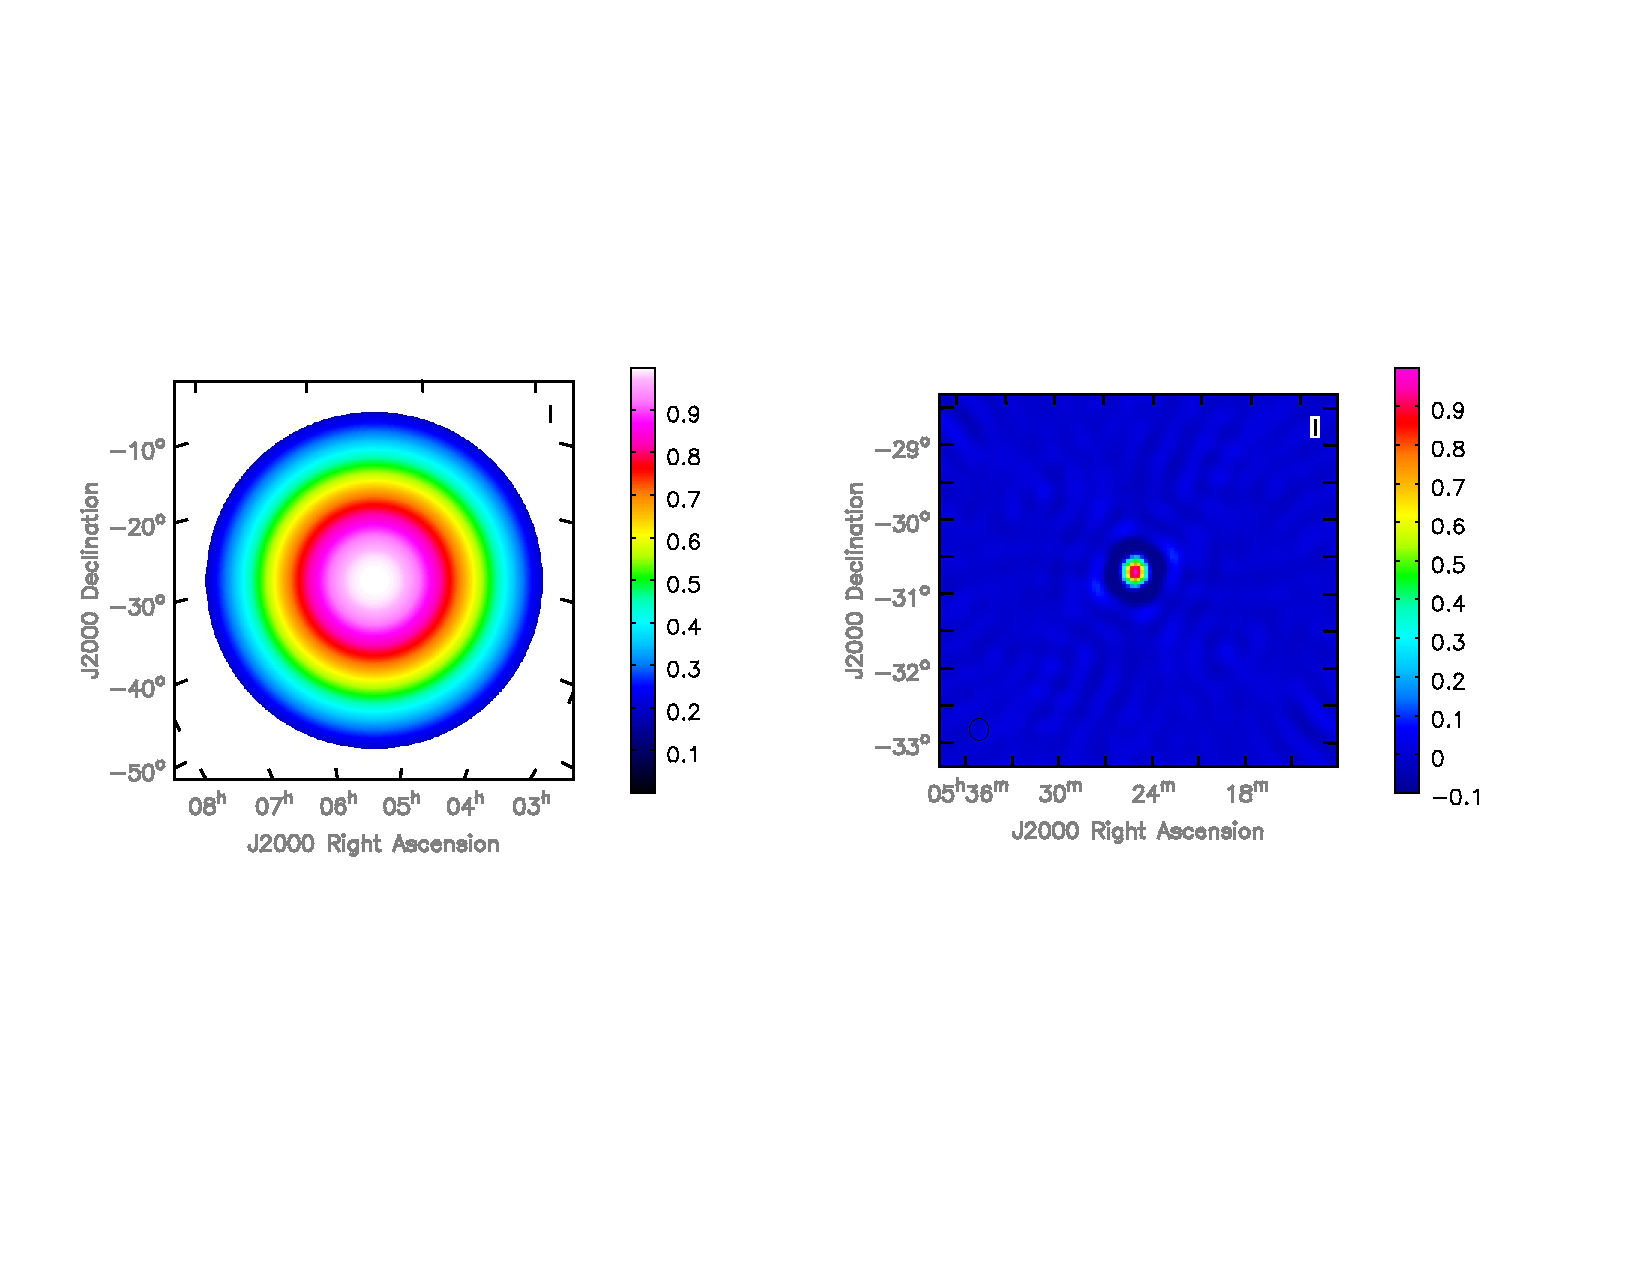
\includegraphics[width=0.8\textwidth]{chapters/polcal/figures/pb_and_psf.pdf}
\caption[The beam model (\textit{left}) and point spread function (\textit{right}) of the PAPER-32 array, calculated by {\tt CASA}.]{The beam model and point spread function of the PAPER-32 array, calculated by {\tt CASA}. In reality, the beam is far less symmetric \citep[e.g.][]{Parsons.10}. The PSF is likely more accurate. Note the difference in axis scales between the two panels.}
\label{figure:polcal_beam_and_psf}
\end{figure}

The times observed by the PAPER-32 imaging array contained the transits of Pictor A and Fornax A. Pictor A is one of the brightest sources in the low frequency sky, is an unresolved point source, and has a simple spectrum \citep{Jacobs.13}:

\begin{equation}
S_{\rm Pic A}(\nu) = 382 \pm 5.4\,{\rm Jy}\,\times\,(\nu/150{\rm MHz})^{-0.76 \pm 0.01},
\end{equation}
making it an ideal flux-calibrator. While it is highly polarized at optical wavelengths \citep[$\sim 50$\%][]{Thomson.95}, it has a low polarization fraction at radio frequencies ($<$5\%; \citet{Perley.97, Huffenberger.15}). Little-to-no expected polarization is useful for obtaining diagonal gains, but a polarized point source is more useful for precisely calculating the off-diagonal \textit{D}-terms (see, for example, Chapter~\ref{chapter:interferometry} or \citet{TMS}). There is a dearth of low-frequency polarized point sources in the low frequency sky \citep{Bernardi.13, Asad.16, Lenc.16}, and only one that is bright enough to be detected by PAPER-32 -- PMN J0351-2744 -- and this we were not able to detect.

To increase the precision of our calibration model, we included a model of Fornax A as well as Pictor A. Fornax A is a bright, resolved radio galaxy which we modelled using three spherical components for its East lobe, West lobe and central core according to MWA observations \citep{McKinley.15}:

\begin{eqnarray}
S_{\rm East}(\nu)= 260\,{\rm Jy}\,\times\,(\nu/154{\rm MHz})^{- 0.77},\\
S_{\rm West}(\nu)= 480\,{\rm Jy}\,\times\,(\nu/154{\rm MHz})^{- 0.77},\\
S_{\rm Core}(\nu)= 12\,{\rm Jy}\,\times\,(\nu/154{\rm MHz})^{- 1.00}.\\
\end{eqnarray}

Fornax A has been found to have a low polarized fraction at higher frequencies \citep[20 GHz][]{Lopez-Caniego.09}, and a $\sim20$\% polarized fraction at 1.51 GHz \citep{Fomalont.89}. \cite{Bernardi.13} found no evidence for polarized emission at 151 MHz using the MWA-32, which may have been partially due to beam depolarization (an effect that would only increase with PAPER-32).

Using this two-source (but with four points) sky model, we used the {\tt CASA} {\tt gaincal} and {\tt bandpass} routines to calibrate a 10 minute snapshot of the transit of Pictor A. We were able to specify a ``Stokes Vector" for each source, and we used $S=(1,0,0,0)$: that is, all components were strictly unpolarized. Applying the calibration solutions and gridding to the \textit{uv}-plane and CLEANing granted the pseudo-Stokes images shown in Figure~\ref{fig:polcal_img_PicA}. As expected, Pictor A dominated the sky in pseudo-Stokes I. However, an excess at its position in the pseudo-Stokes Q image suggested a mis-calibration in the diagonal gains at the $\sim10$\% level. No sources are visible above the noise in pseudo-Stokes U and V. However, these parameters (as well as pseudo-Stokes Q) exhibited a high fringe-rate oscillation in the North-West to South-East direction, which suggested that a long baseline of that orientation was poorly calibrated, or the antenna was malfunctioning. A similar effect was seen with a low fringe-rate from North-East to South-West, suggesting a problem on a short baseline with that orientation. Indeed, \cite{Kohn.16} found three malfunctioning antennas during their study using the PAPER-32 imaging array, which match the orientation and lengths indicated by the fringing (see Chapter~\ref{chapter:eor_window_paper32img}, Figure~\ref{fig:psa32img_config}). Removing those antennas resulted in cleaner images with lower noise-floors, as shown in Figure~\ref{fig:polcal_img_PicA_improved}. New fringing is seen at various angles, the source of which would be more difficult to identify. Excesses at the position of Pictor A in pseudo-Stokes U and V are likely the result of uncalibrated D-terms, which will be addressed in Section~\ref{subsec:polcal_Dterms}.
The morphology of point sources in pseudo-Stokes I matched the PSF shown in Figure~\ref{figure:polcal_beam_and_psf}, showing that the CLEAN algorithm converged when during imaging.

\begin{figure}
\hspace{-2cm}\begin{tabular}{ll}
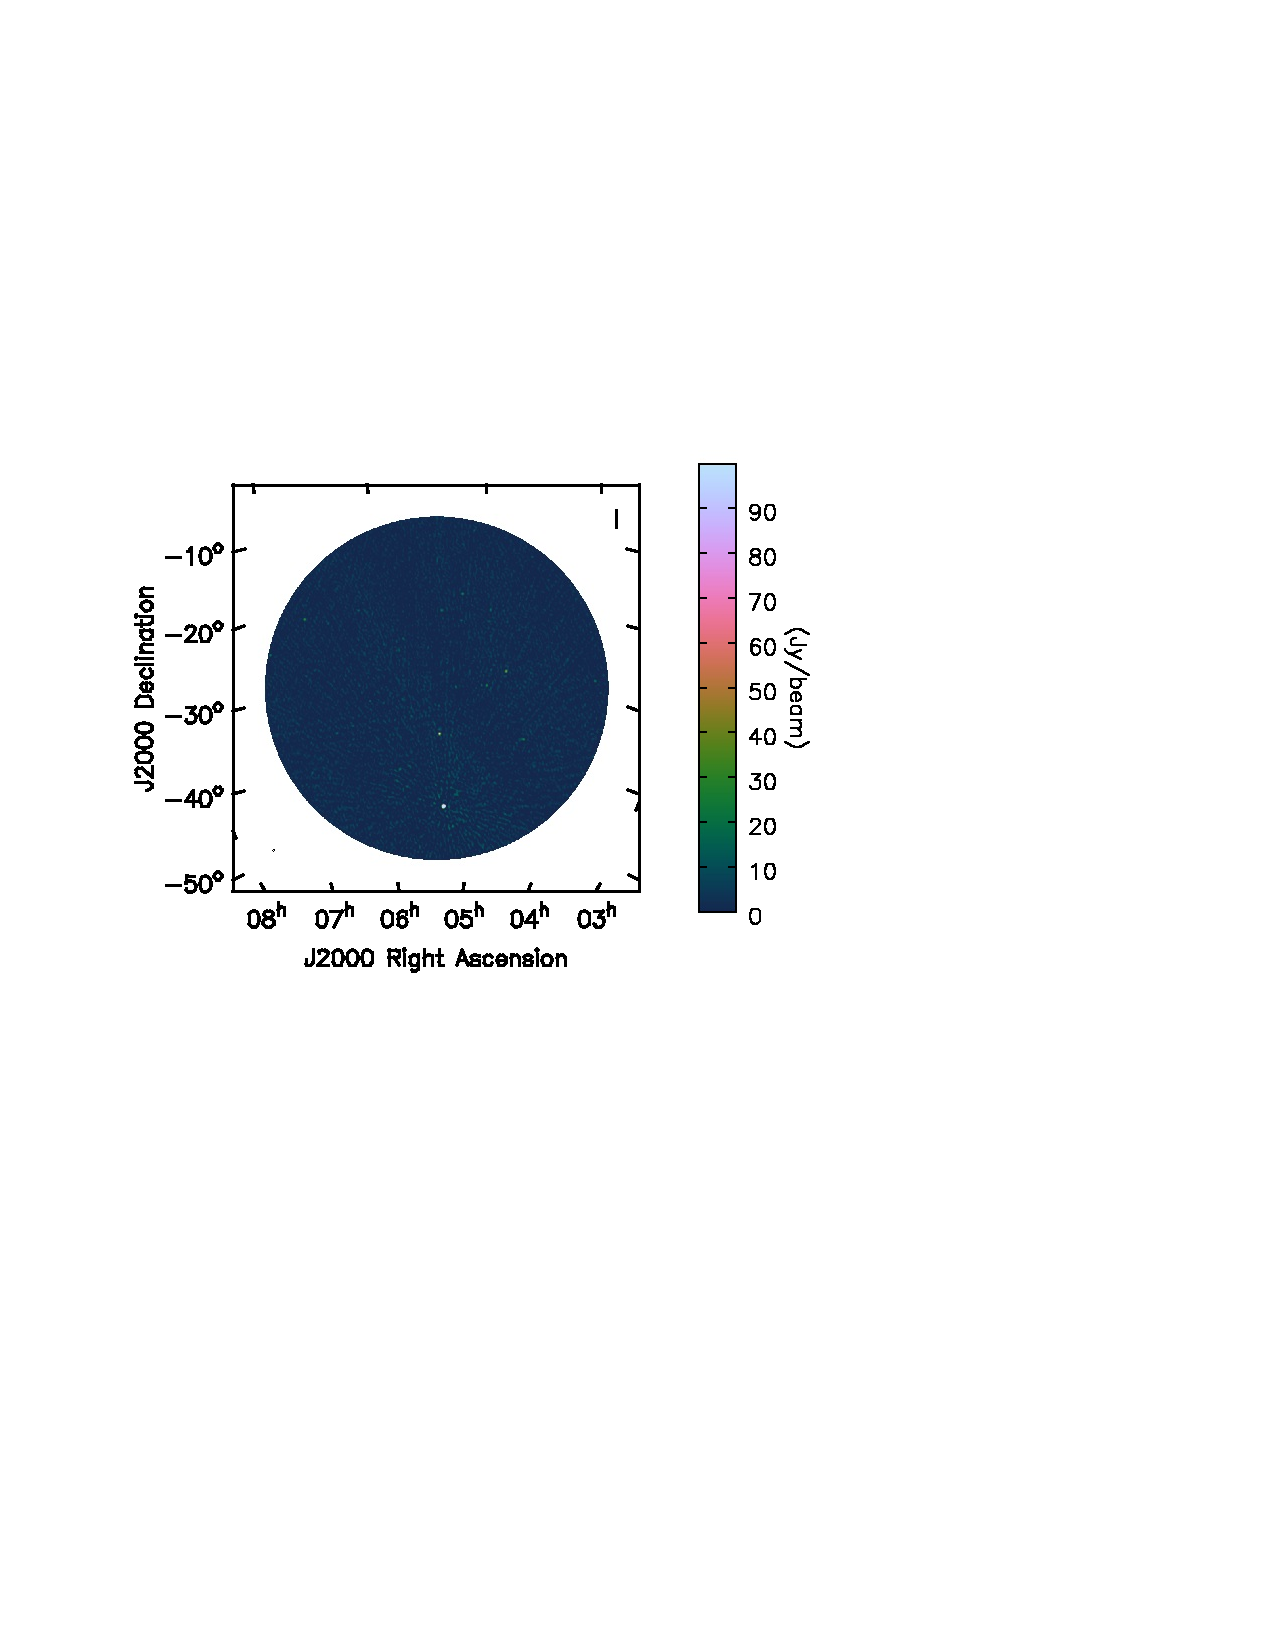
\includegraphics[clip, trim=0.1cm 11cm 6cm 6cm, width=0.6\textwidth]{chapters/polcal/figures/68380-I.pdf} &
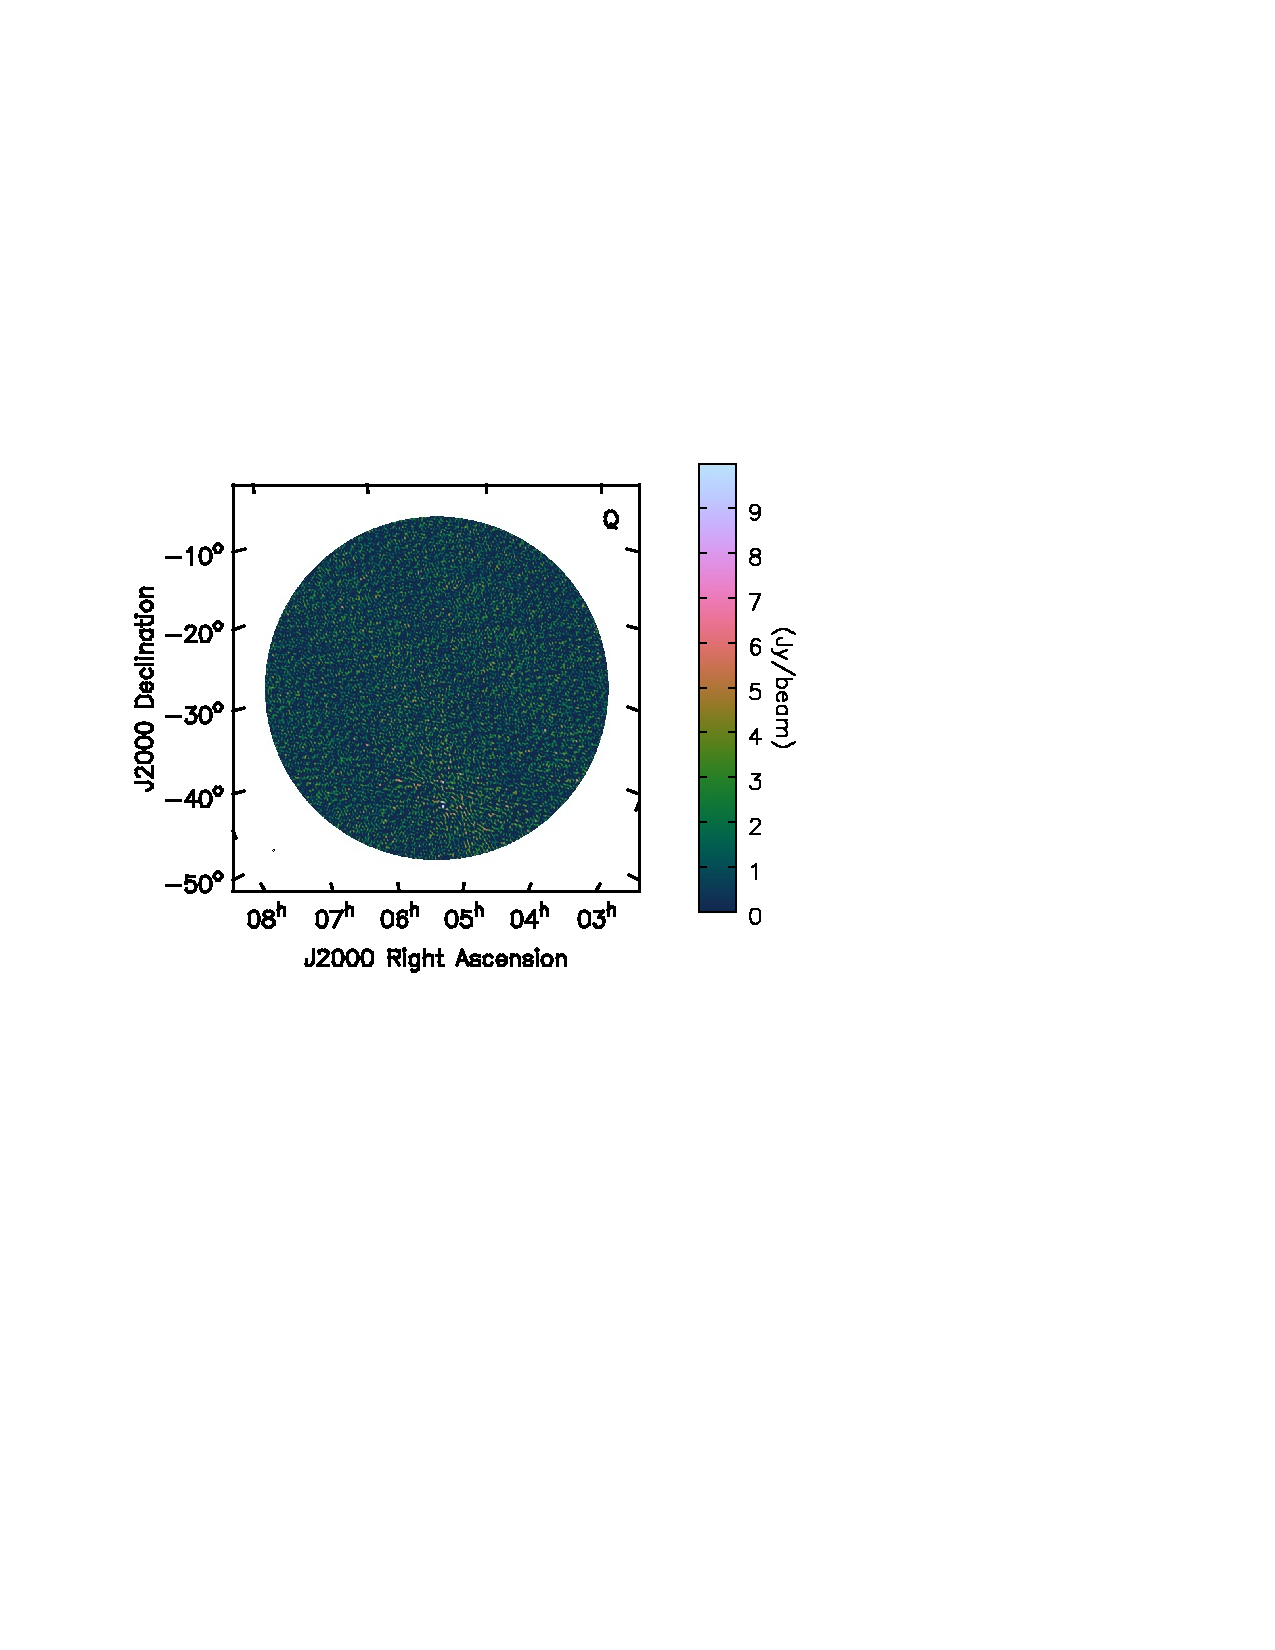
\includegraphics[clip, trim=0.1cm 11cm 6cm 6cm, width=0.6\textwidth]{chapters/polcal/figures/68380-Q.pdf} \\
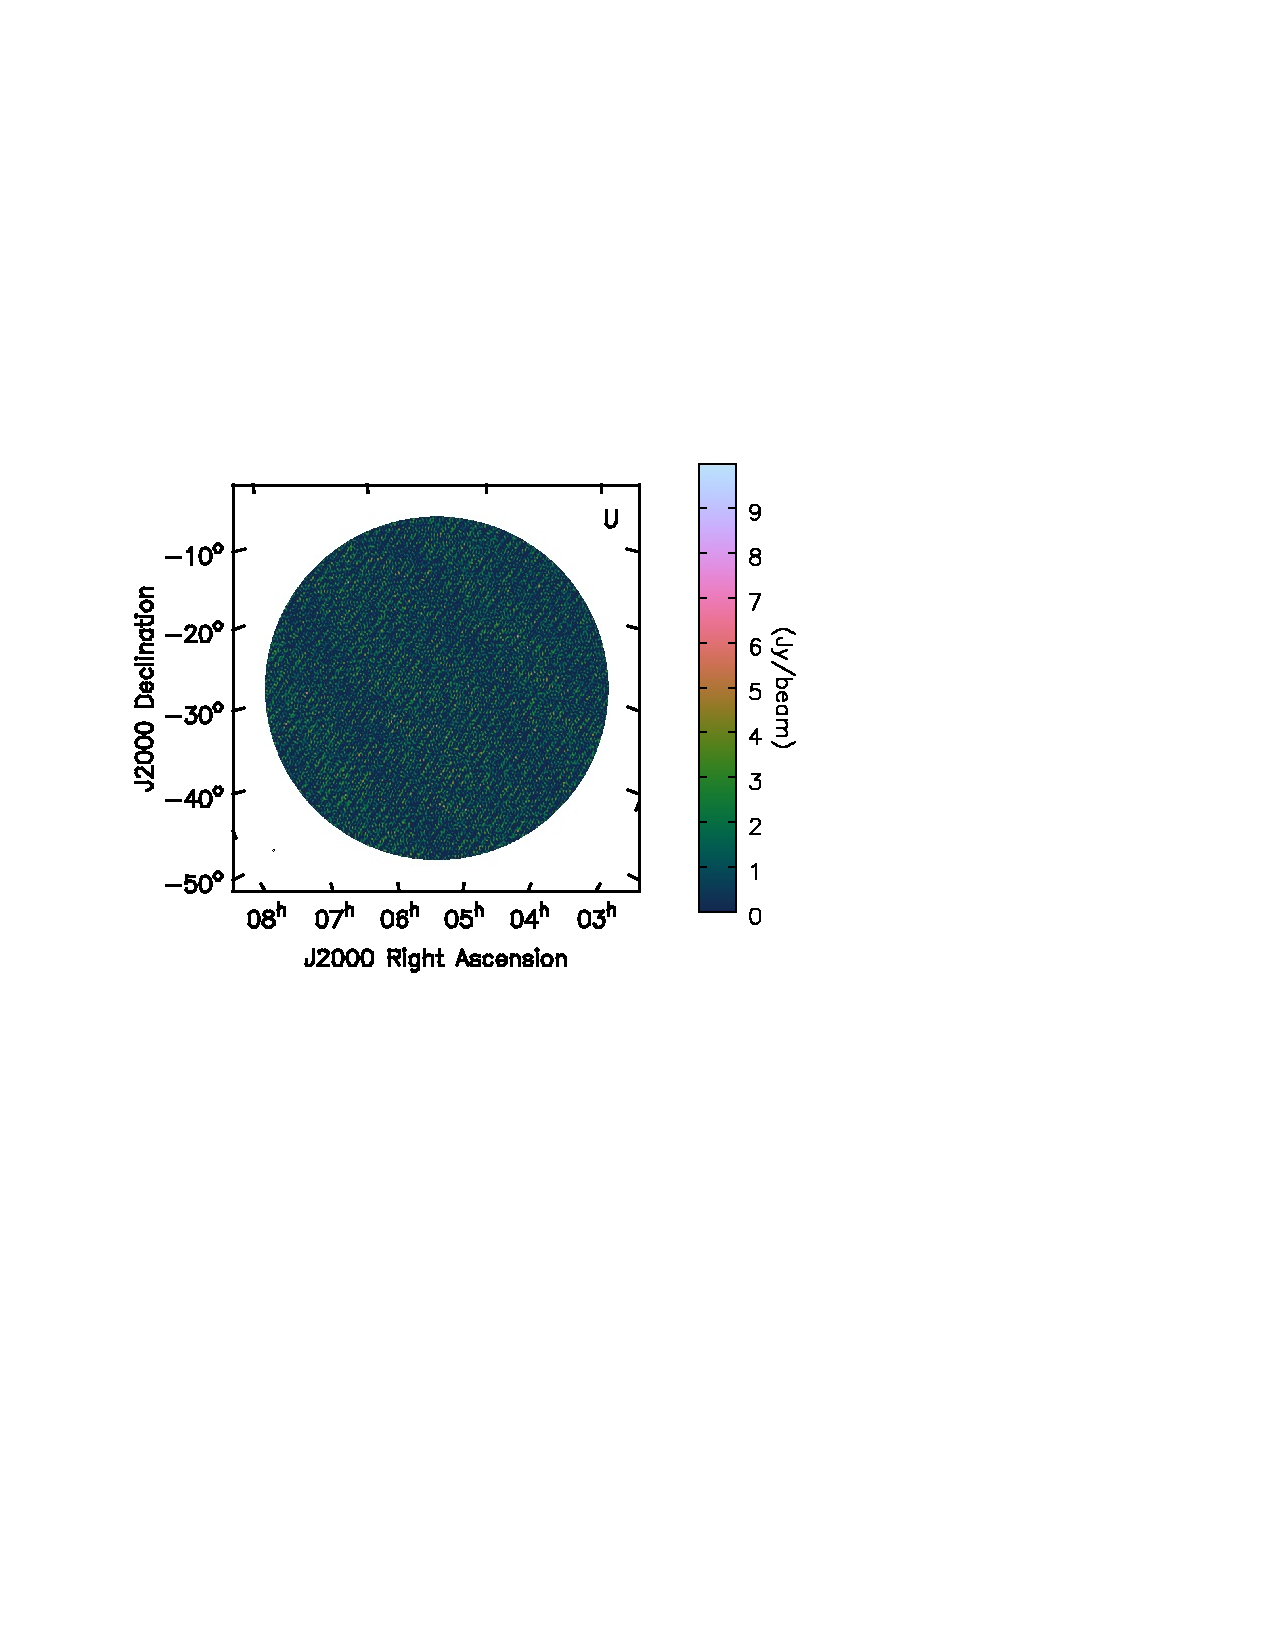
\includegraphics[clip, trim=0.1cm 11cm 6cm 6cm, width=0.6\textwidth]{chapters/polcal/figures/68380-U.pdf} &
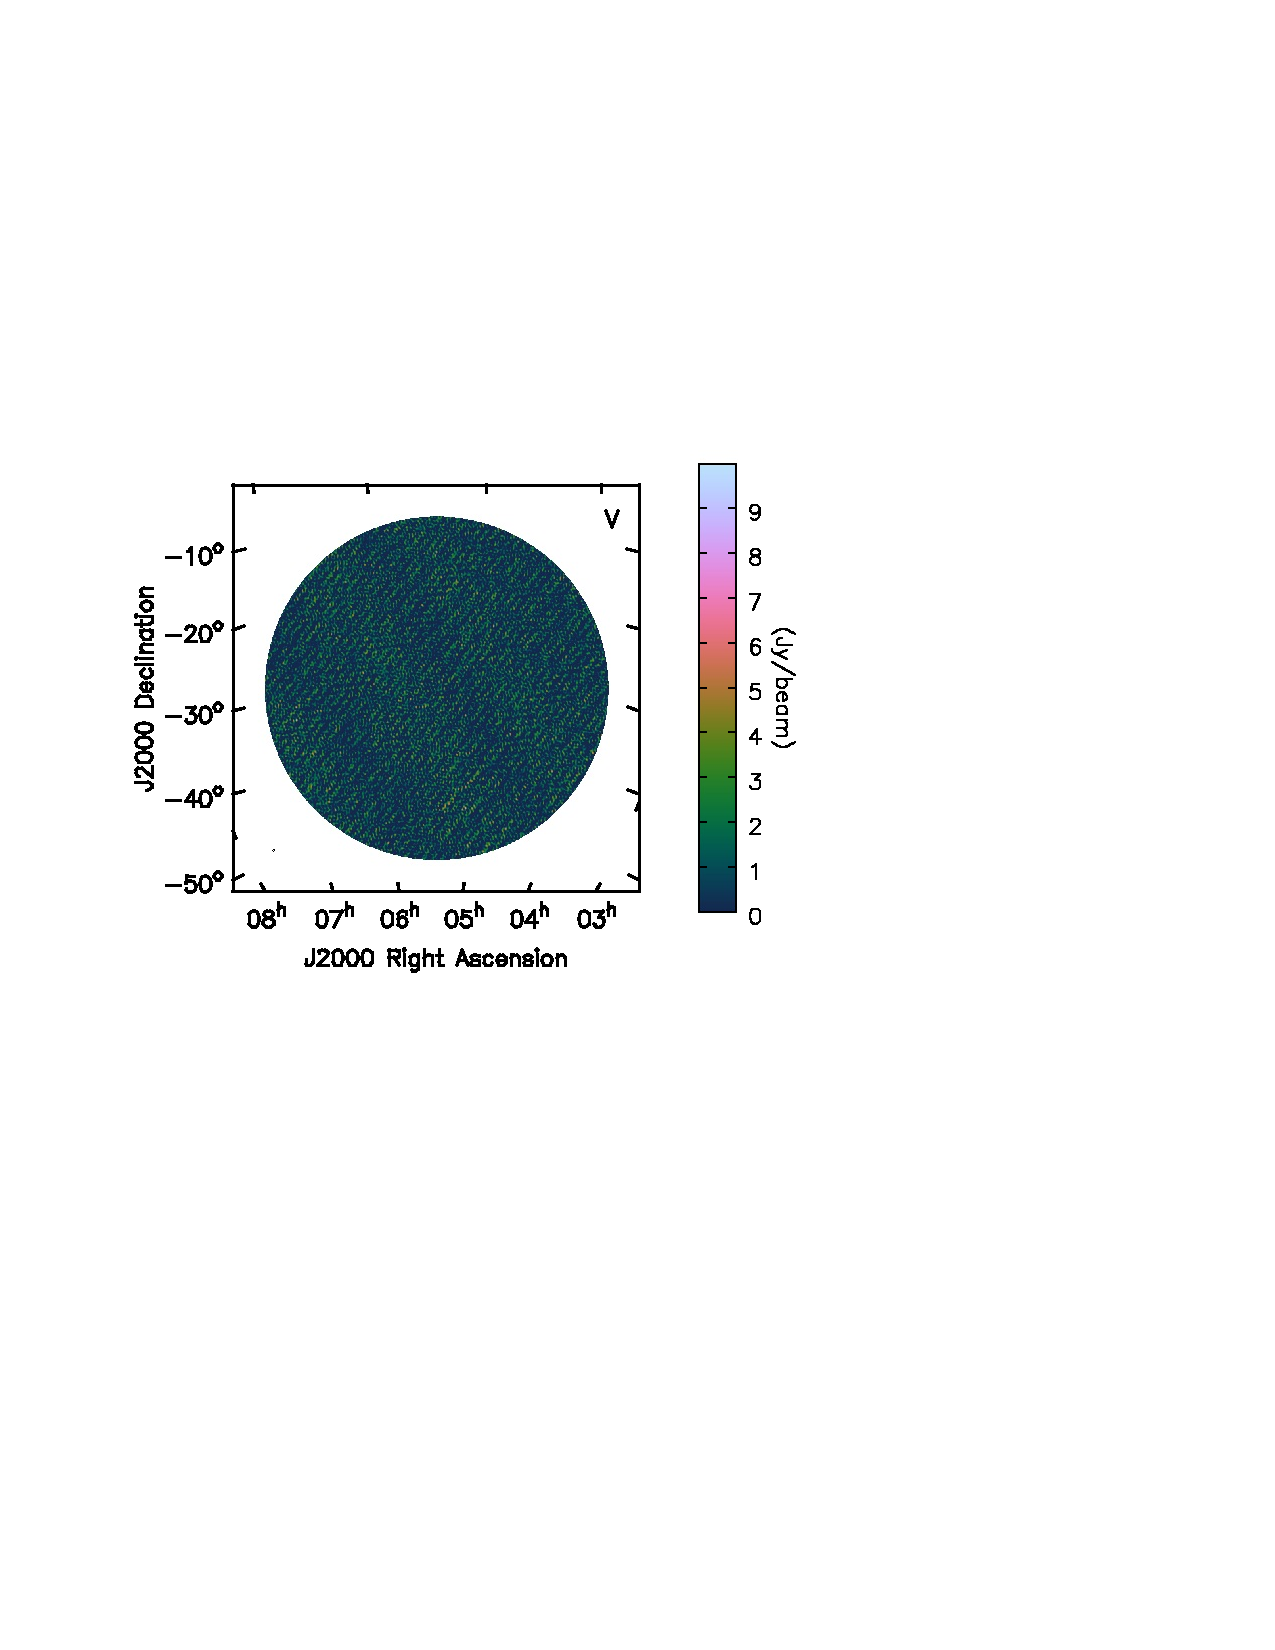
\includegraphics[clip, trim=0.1cm 11cm 6cm 6cm, width=0.6\textwidth]{chapters/polcal/figures/68380-V.pdf} \\
\end{tabular}
\caption[Full-polarization imaging results from a four-component, Stokes I-only sky model.]{Full-polarization imaging results from a four-component, Stokes I-only sky model. Images are multi-frequency syntheses from 110 to 180 MHz. Pictor A, the brightest unresolved source in the Southern Sky at our frequencies, is in transit and dominates the sky in pseudo-Stokes I. An excess in pseudo-Stokes Q at the $\sim10$\% level indicates inaccuracies in the gain calibration. Pseudo-Stokes U and V are noise-like, save for a fringe that rises above the noise -- indicating a poor calibration of a single baseline of that orientation.}
\label{fig:polcal_img_PicA}
\end{figure}

\begin{figure}
\hspace{-2cm}\begin{tabular}{ll}
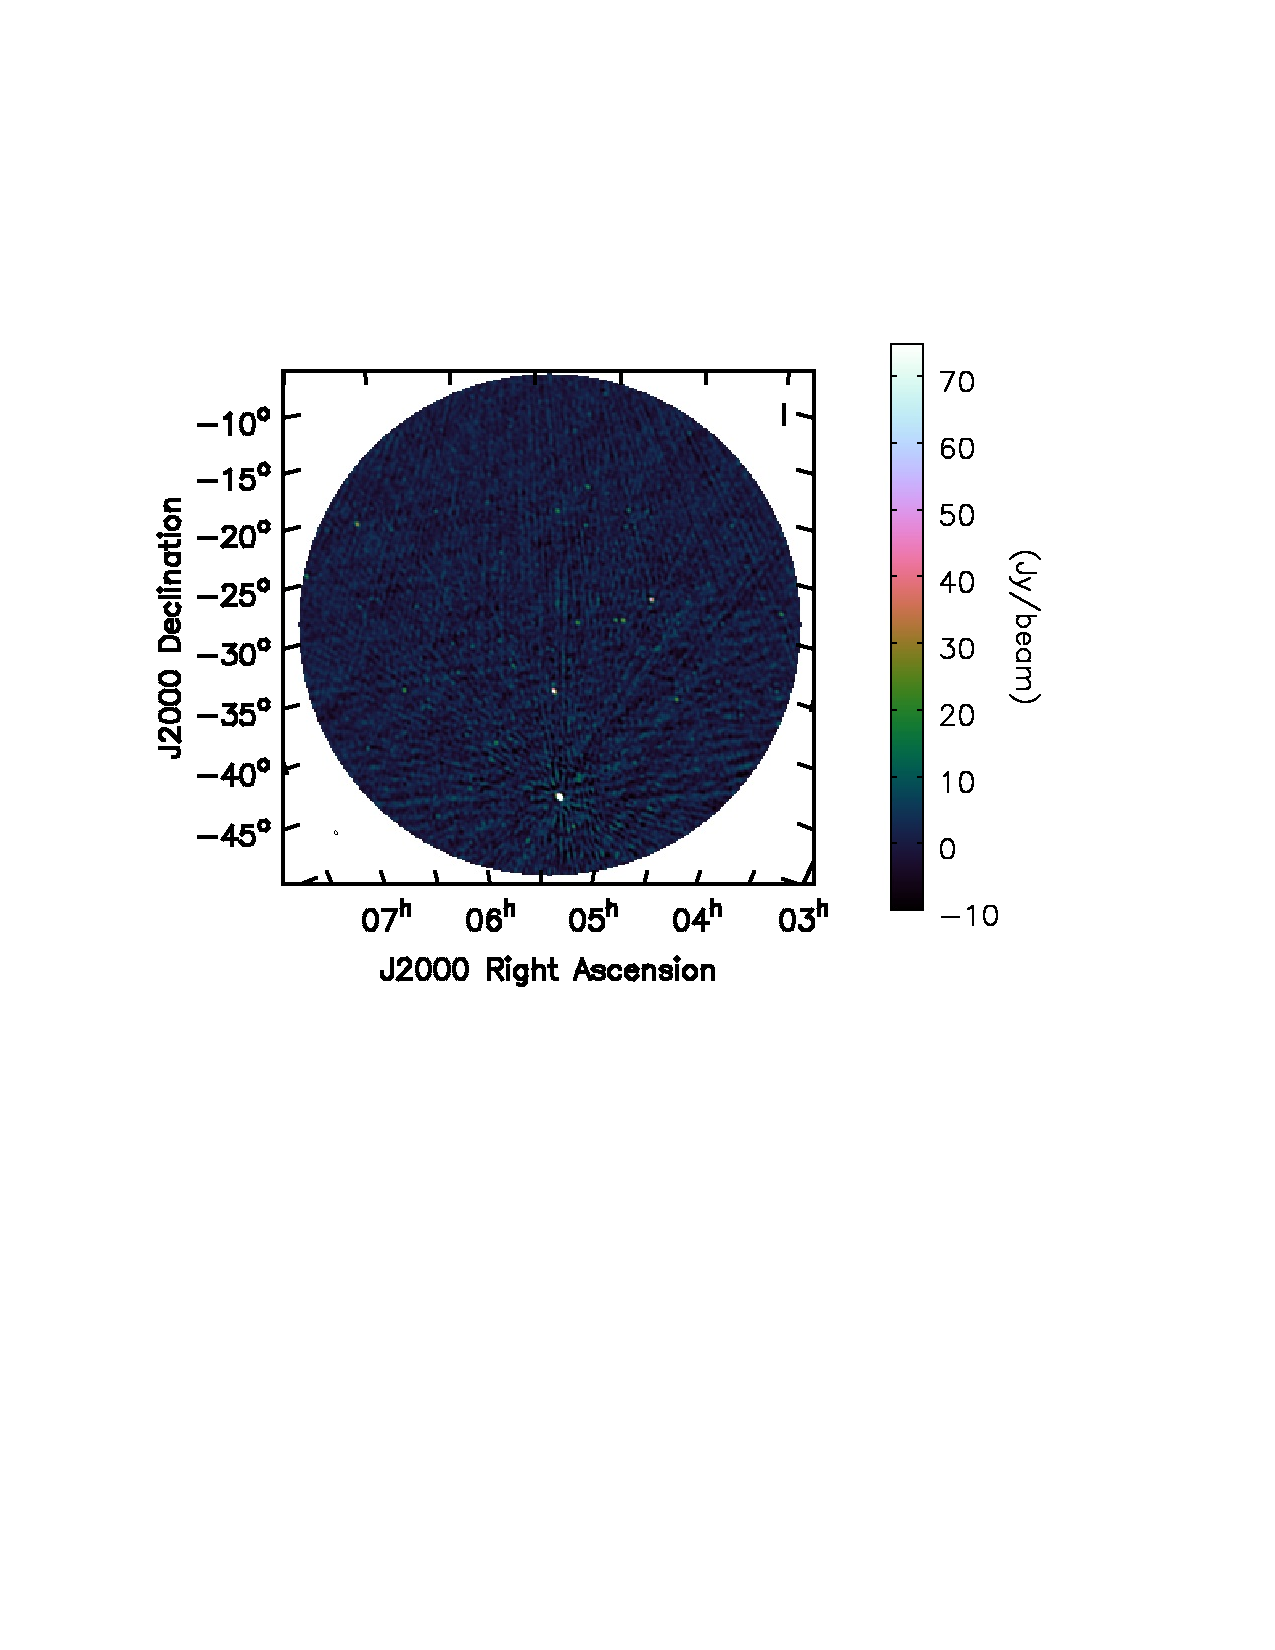
\includegraphics[clip, trim=0.5cm 11cm 4cm 5cm, width=0.6\textwidth]{chapters/polcal/figures/68380-I-better.pdf} &
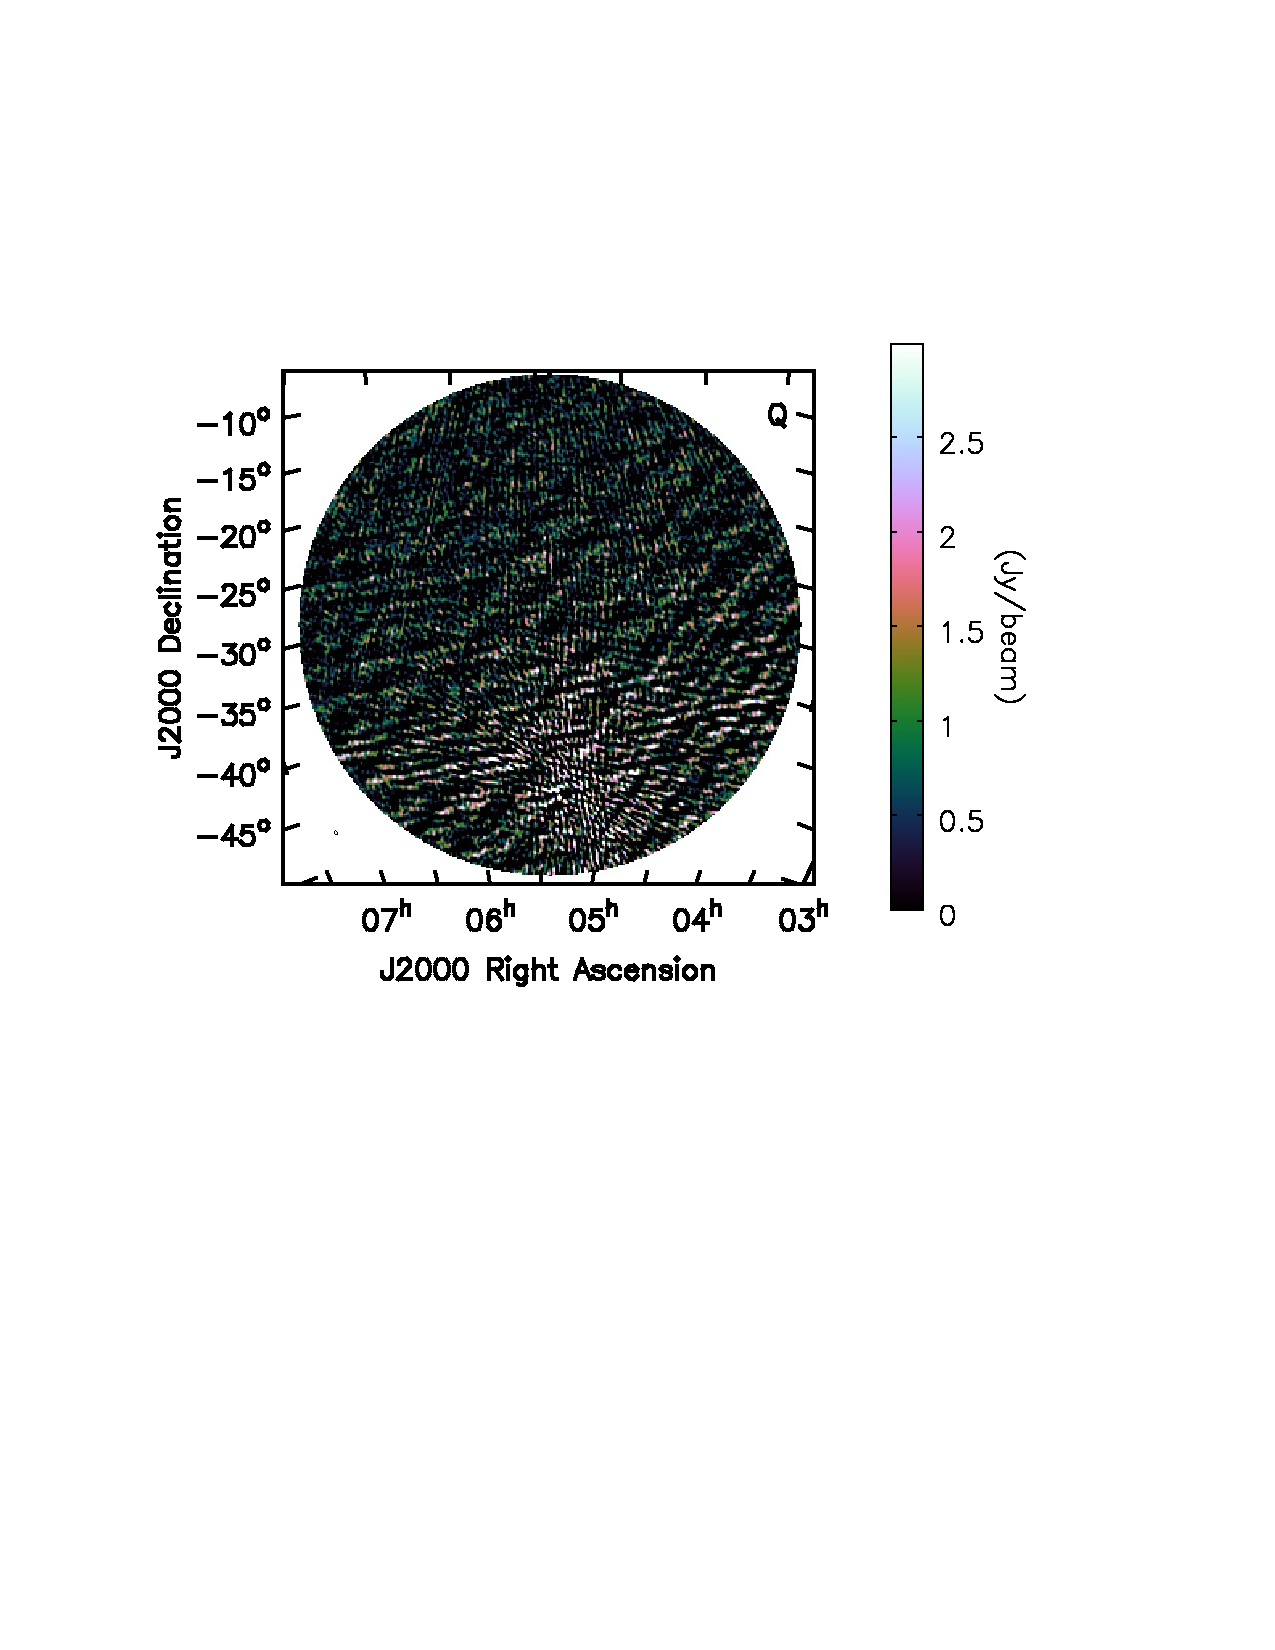
\includegraphics[clip, trim=0.5cm 11cm 4cm 5cm, width=0.6\textwidth]{chapters/polcal/figures/68380-Q-better.pdf} \\
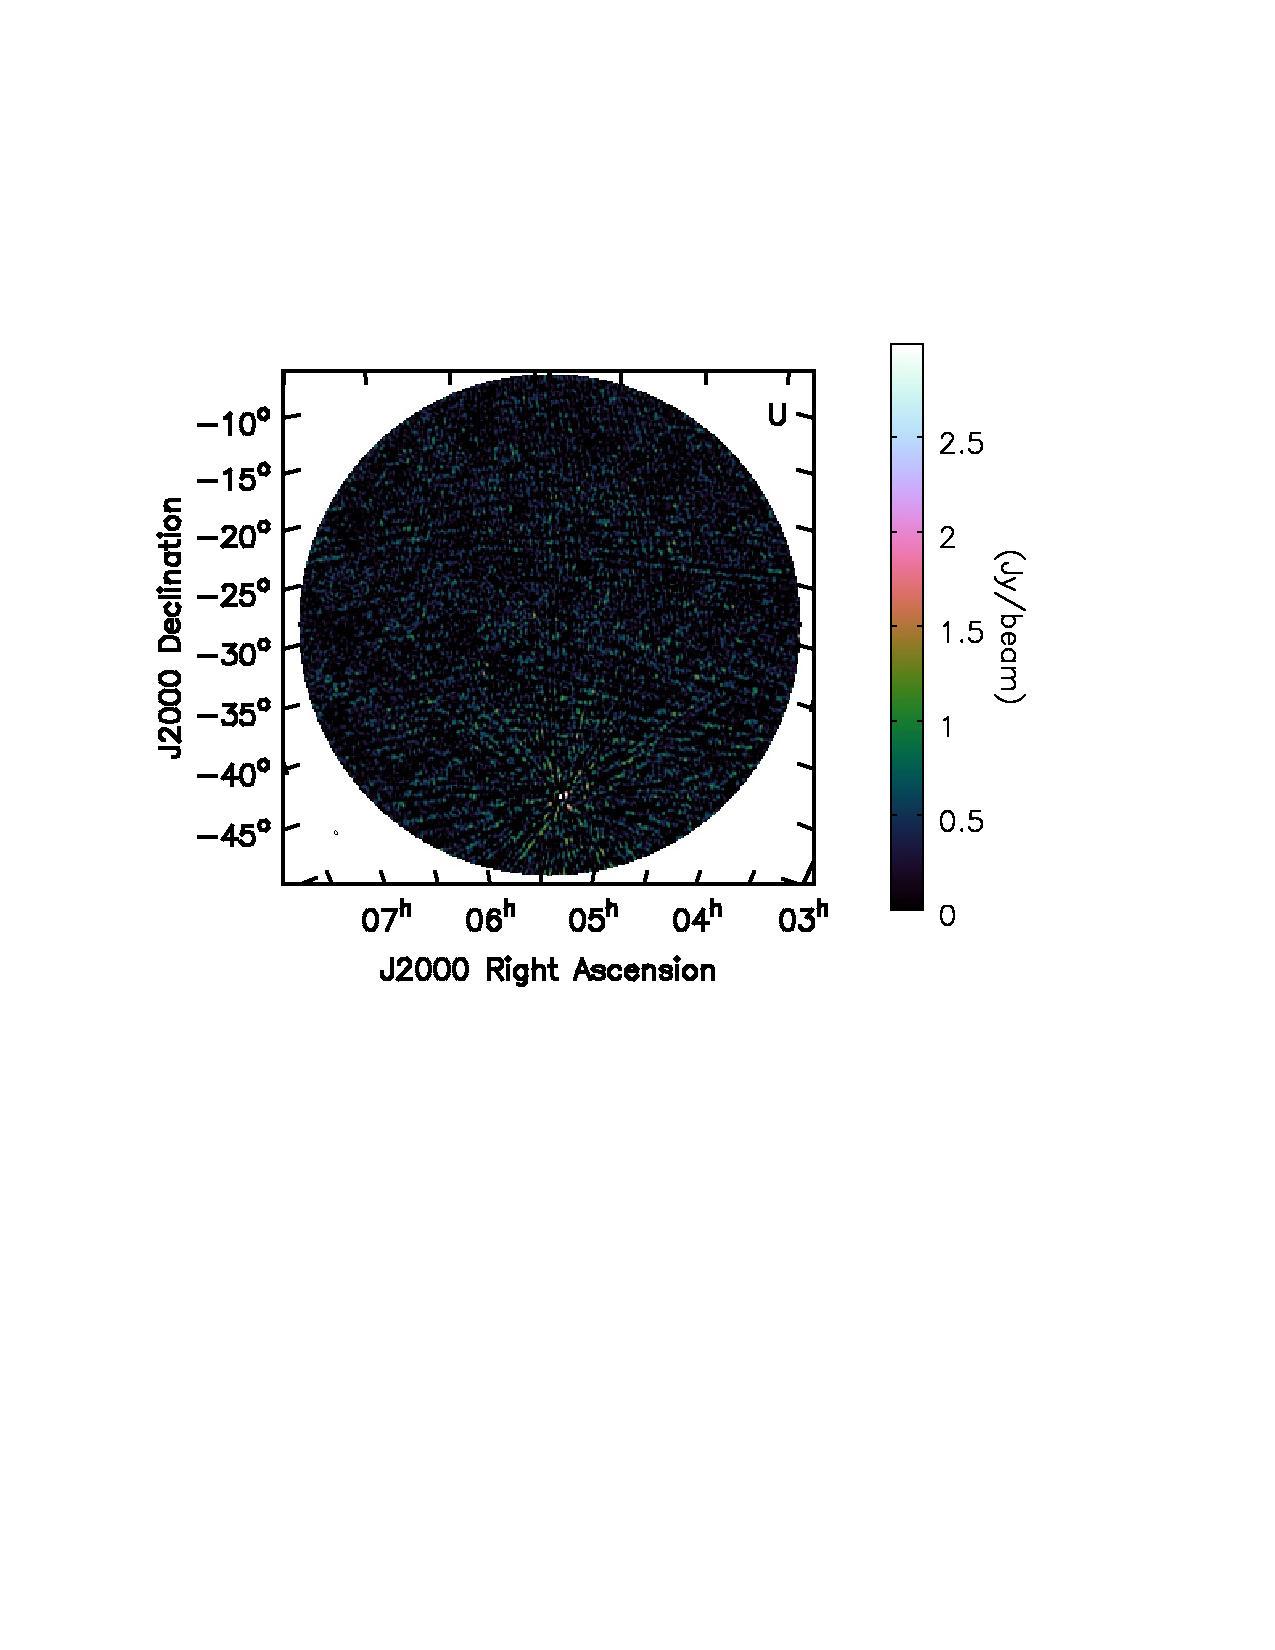
\includegraphics[clip, trim=0.5cm 11cm 4cm 5cm, width=0.6\textwidth]{chapters/polcal/figures/68380-U-better.pdf} &
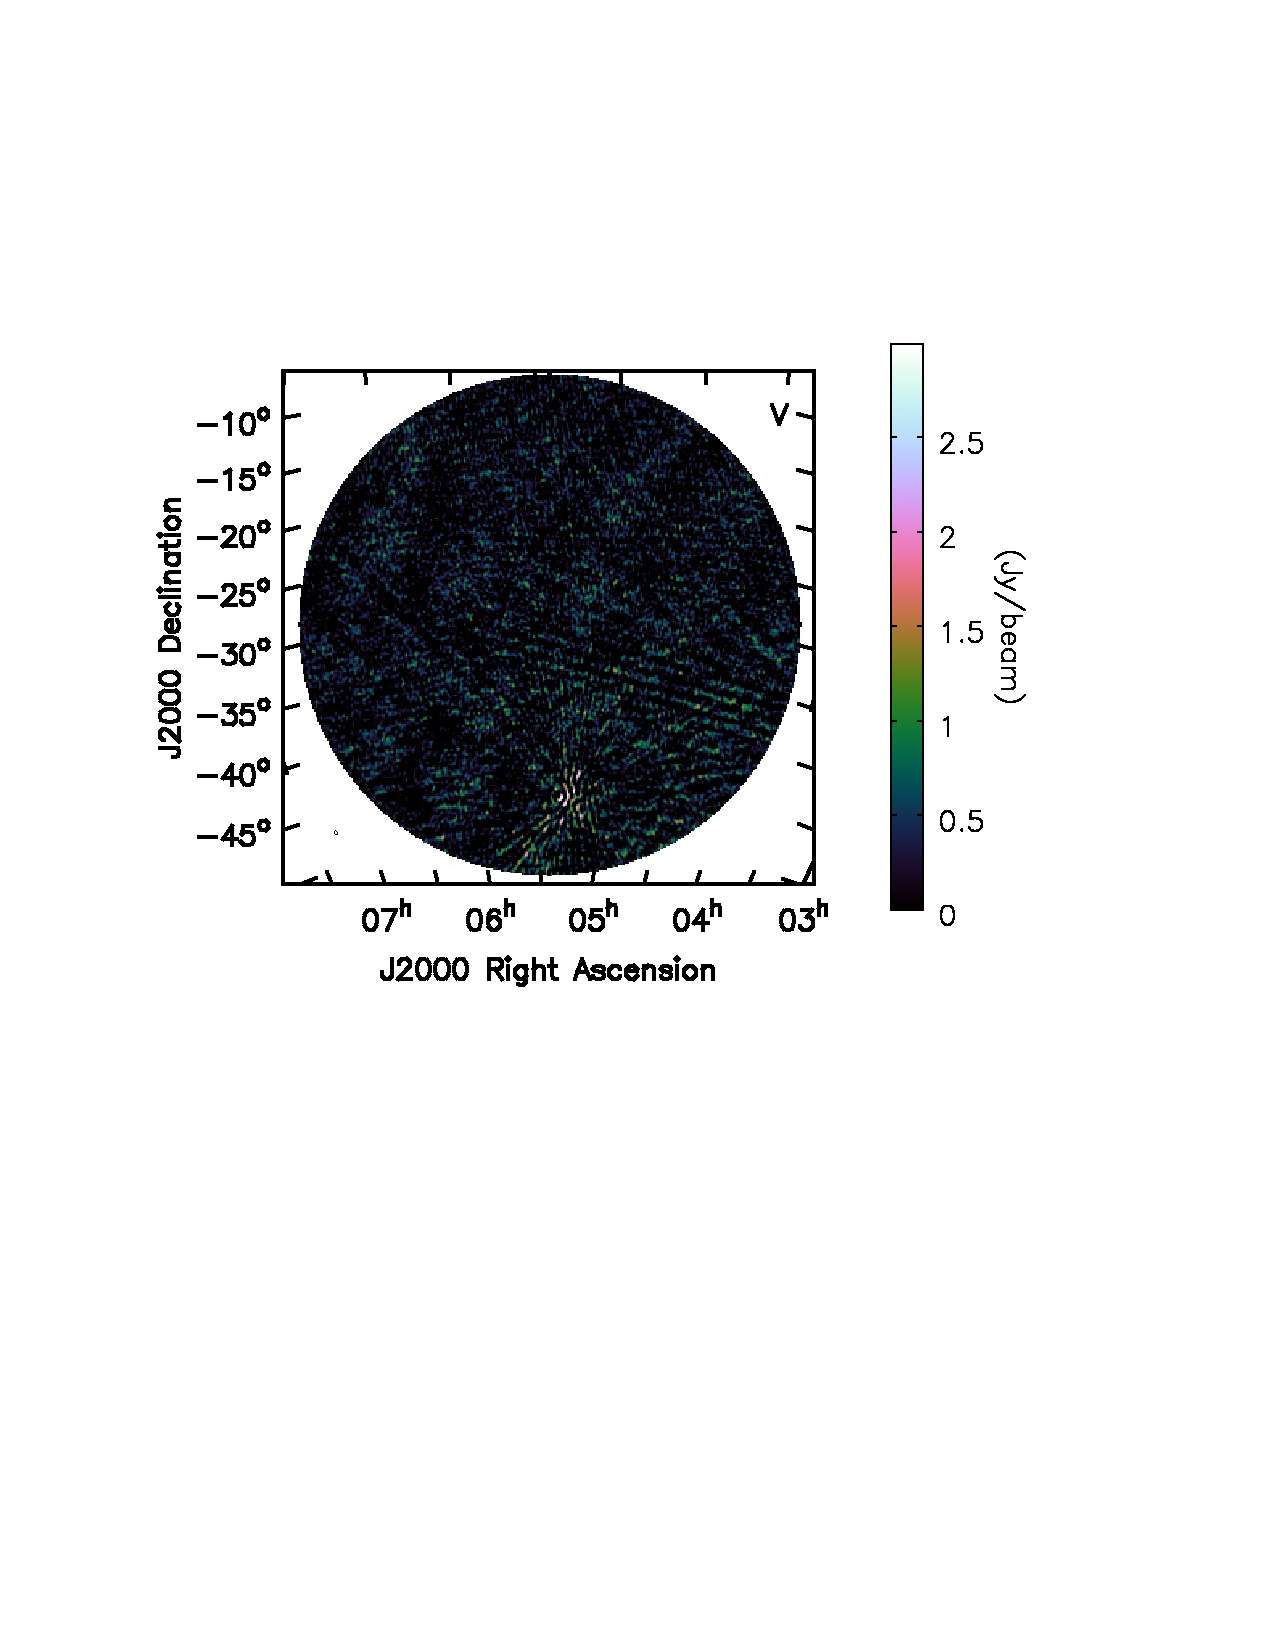
\includegraphics[clip, trim=0.5cm 11cm 4cm 5cm, width=0.6\textwidth]{chapters/polcal/figures/68380-V-better.pdf} \\
\end{tabular}
\caption[The same field as shown in Figure~\ref{fig:polcal_img_PicA}, but with the removal of malfunctioning antennas identified by \cite{Kohn.16}.]{The same field as shown in Figure~\ref{fig:polcal_img_PicA}, but with the removal of malfunctioning antennas identified by \cite{Kohn.16}. The noise level drops and much of the fringing in pseudo-Stokes Q, U and V disappears (note the change in color scales and zoom level).}
\label{fig:polcal_img_PicA_improved}
\end{figure}

We were able to test the stability of the instrument by applying the calibration solutions derived from the Pictor A transit to a completely different field. The imaging results of such a test at LST$\approx$0.5 hours are shown in Figure~\ref{fig:polcal_img_LST05}. The pseudo-Stokes I image showed a point-source dominated field, as expected for this LST, and pseudo-Stokes Q, U and V were dominated by noise. These results were proof of instrument stability in time at the $\sim$6 hour level.

\begin{figure}
\hspace{-2cm}\begin{tabular}{ll}
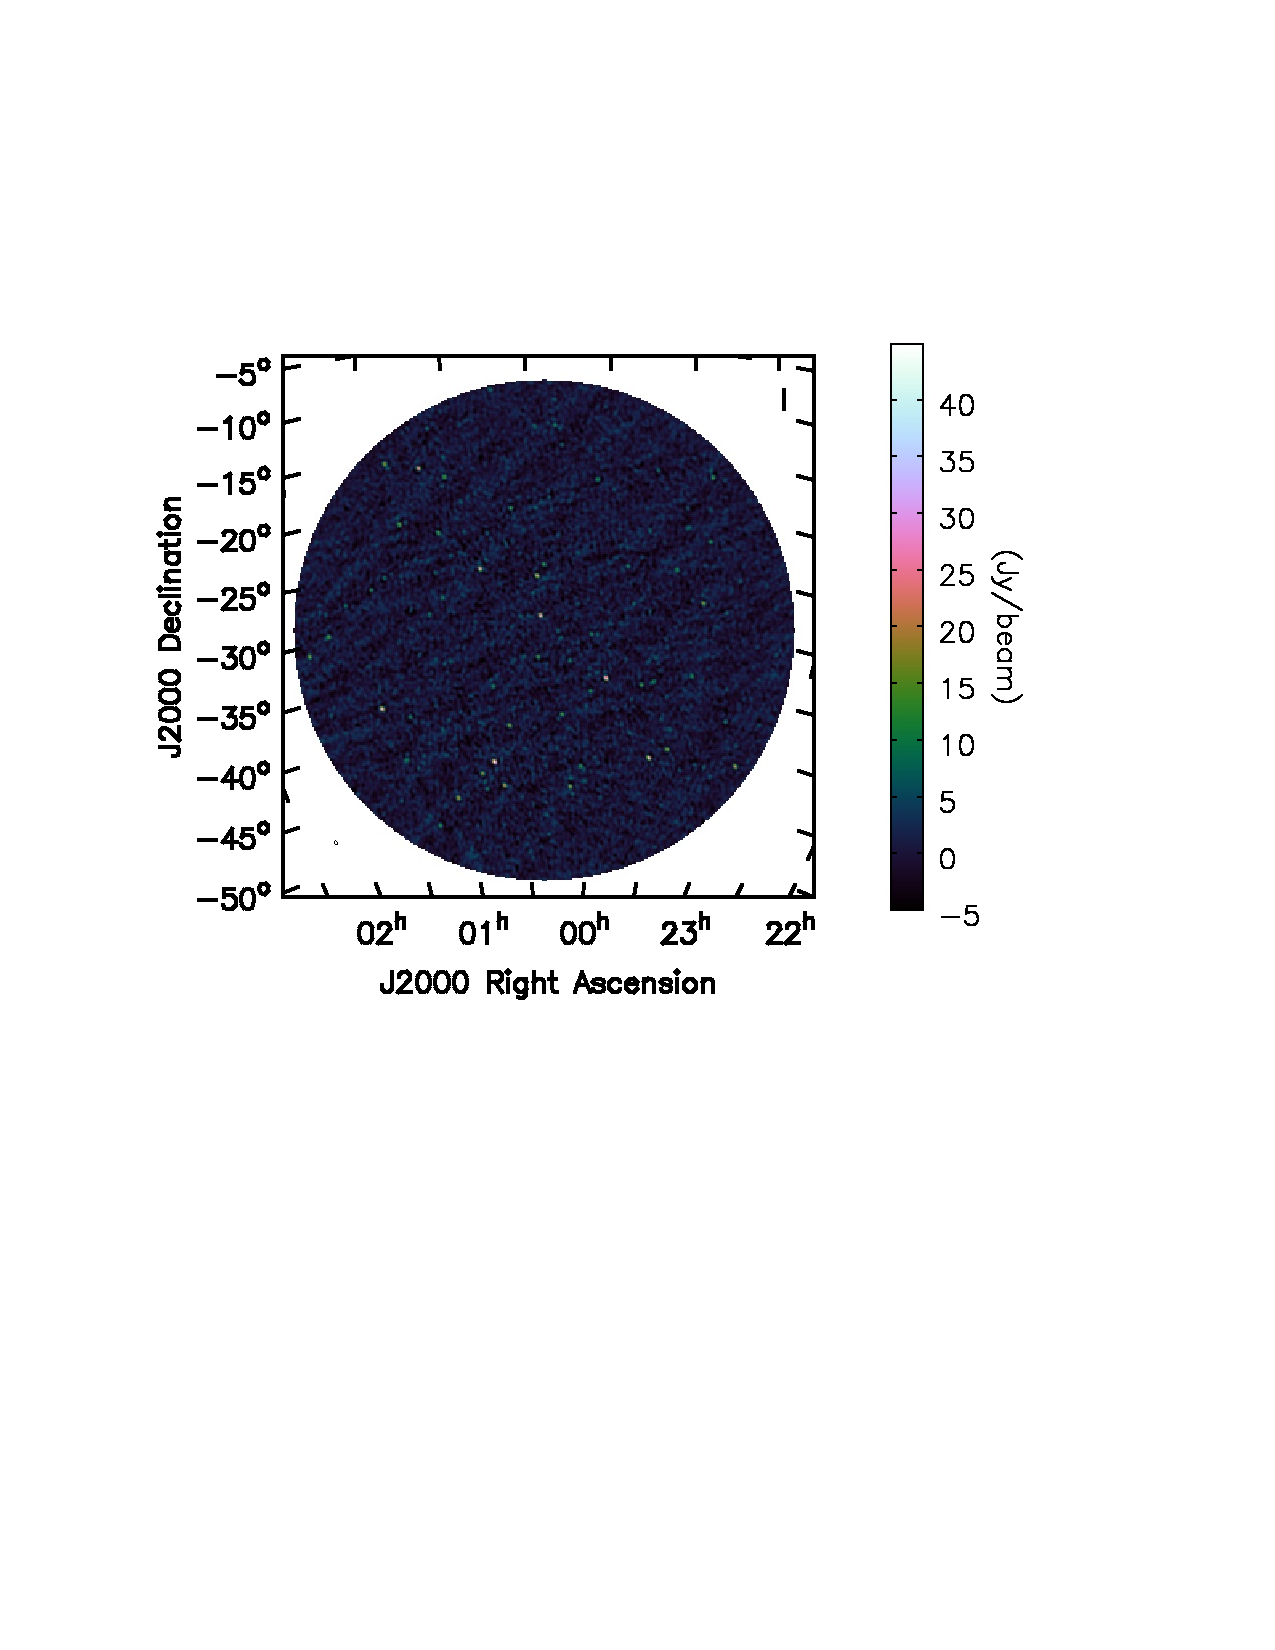
\includegraphics[clip, trim=0.5cm 11cm 3cm 5cm, width=0.6\textwidth]{chapters/polcal/figures/47501-I-better.pdf} &
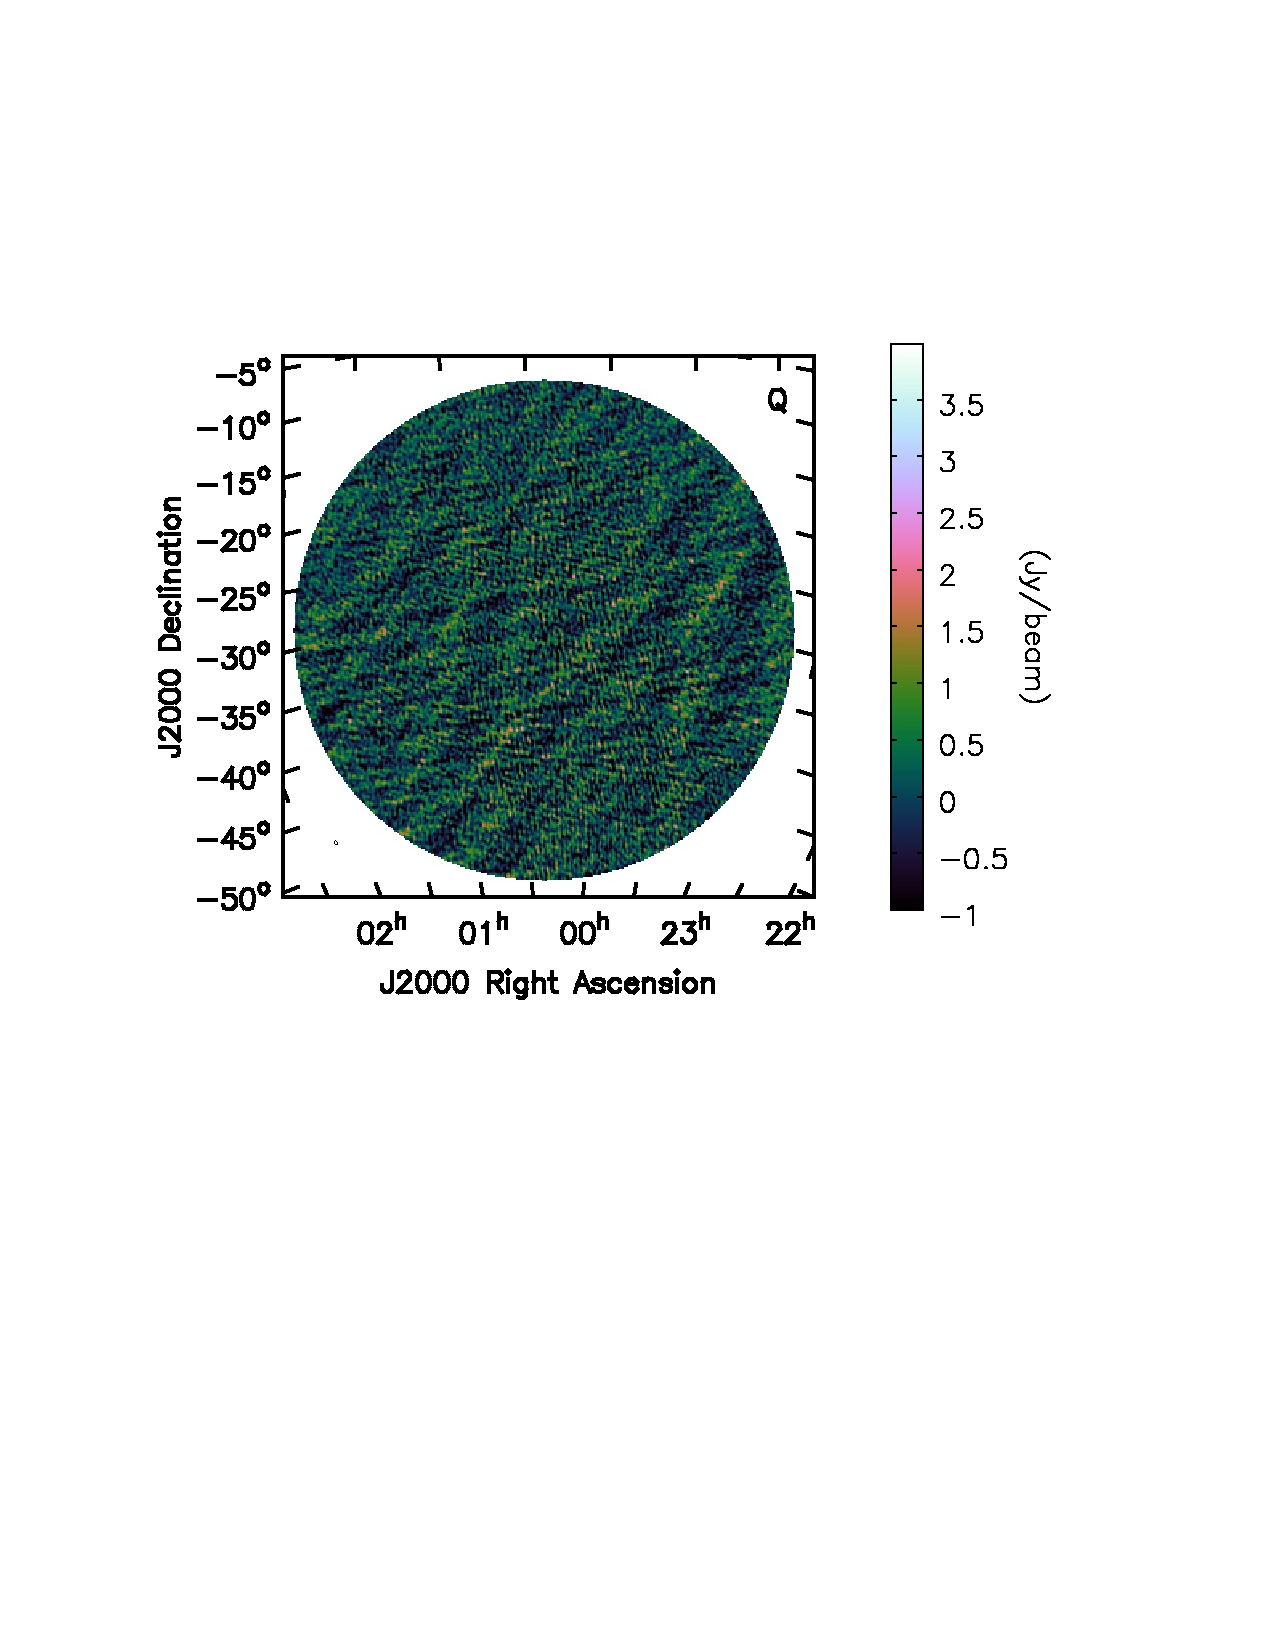
\includegraphics[clip, trim=0.5cm 11cm 3cm 5cm, width=0.6\textwidth]{chapters/polcal/figures/47501-Q-better.pdf} \\
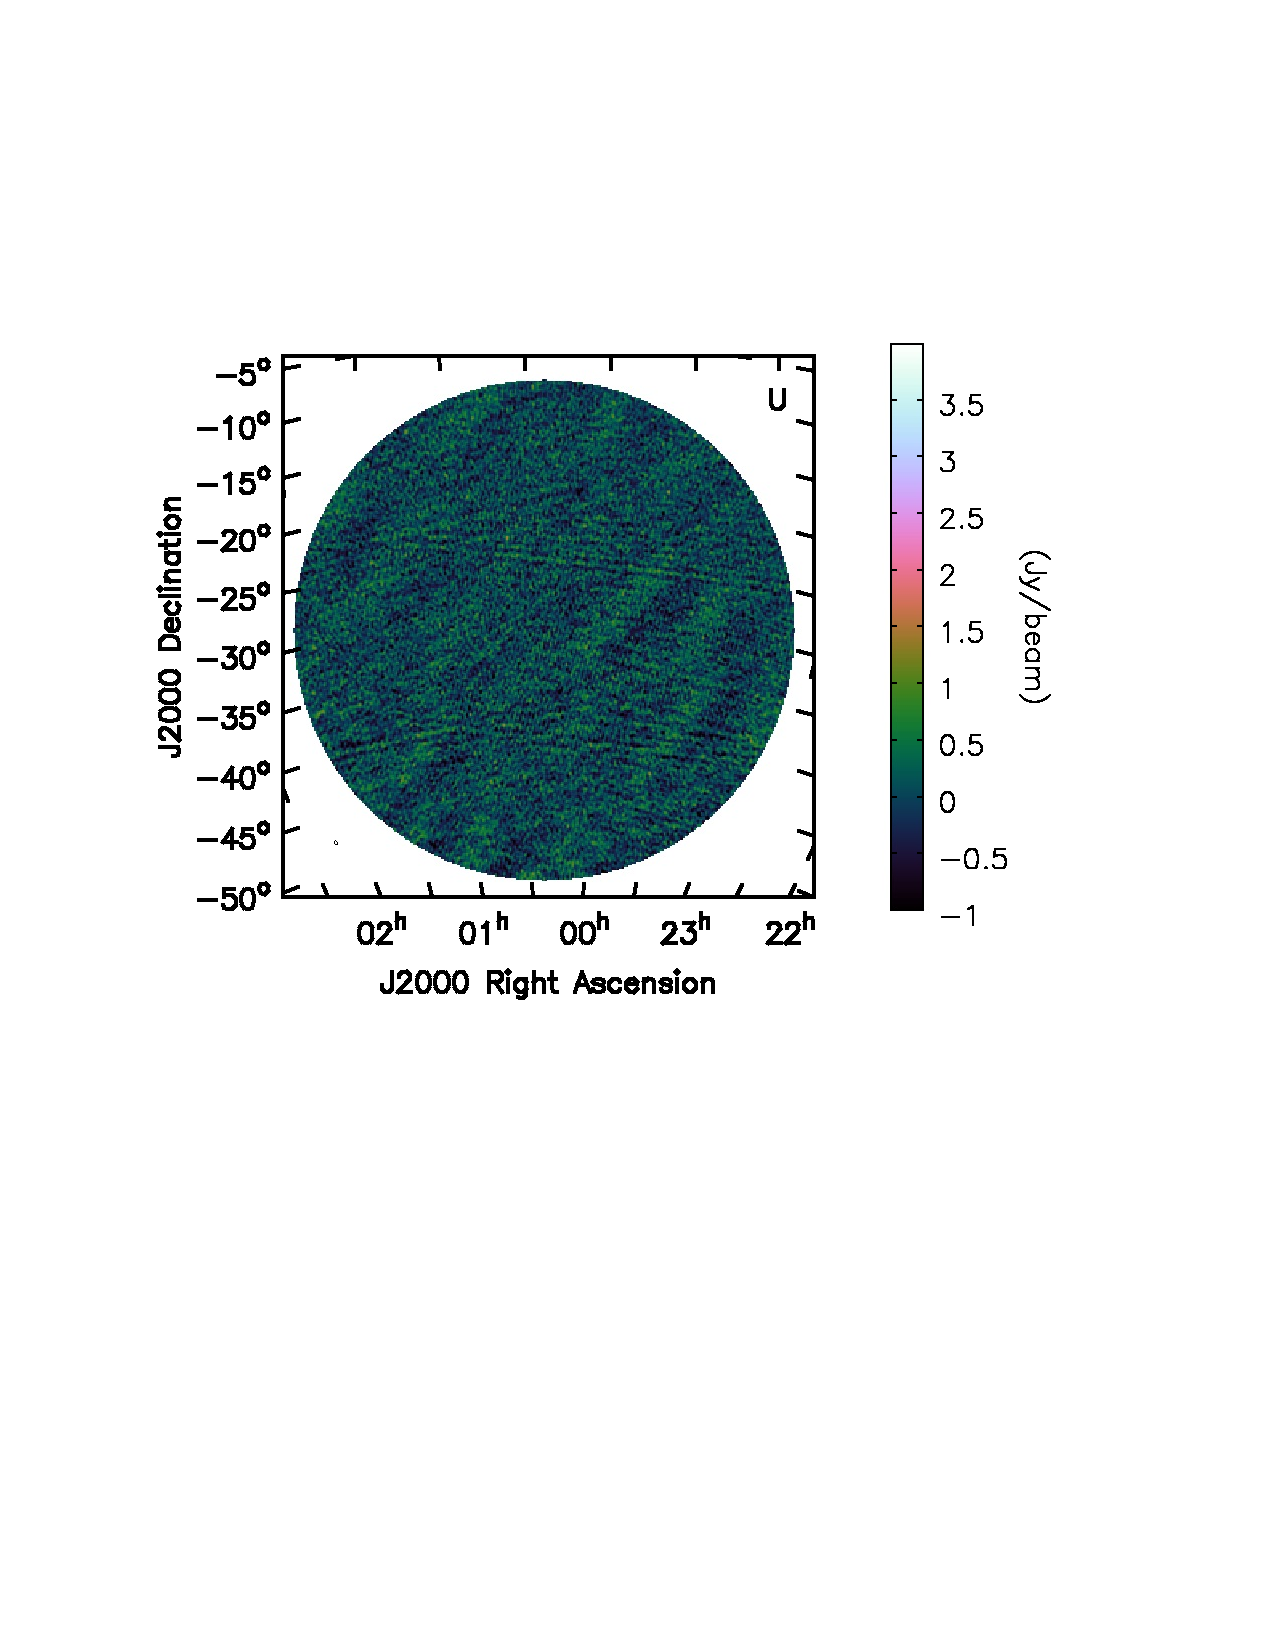
\includegraphics[clip, trim=0.5cm 11cm 3cm 5cm, width=0.6\textwidth]{chapters/polcal/figures/47501-U-better.pdf} &
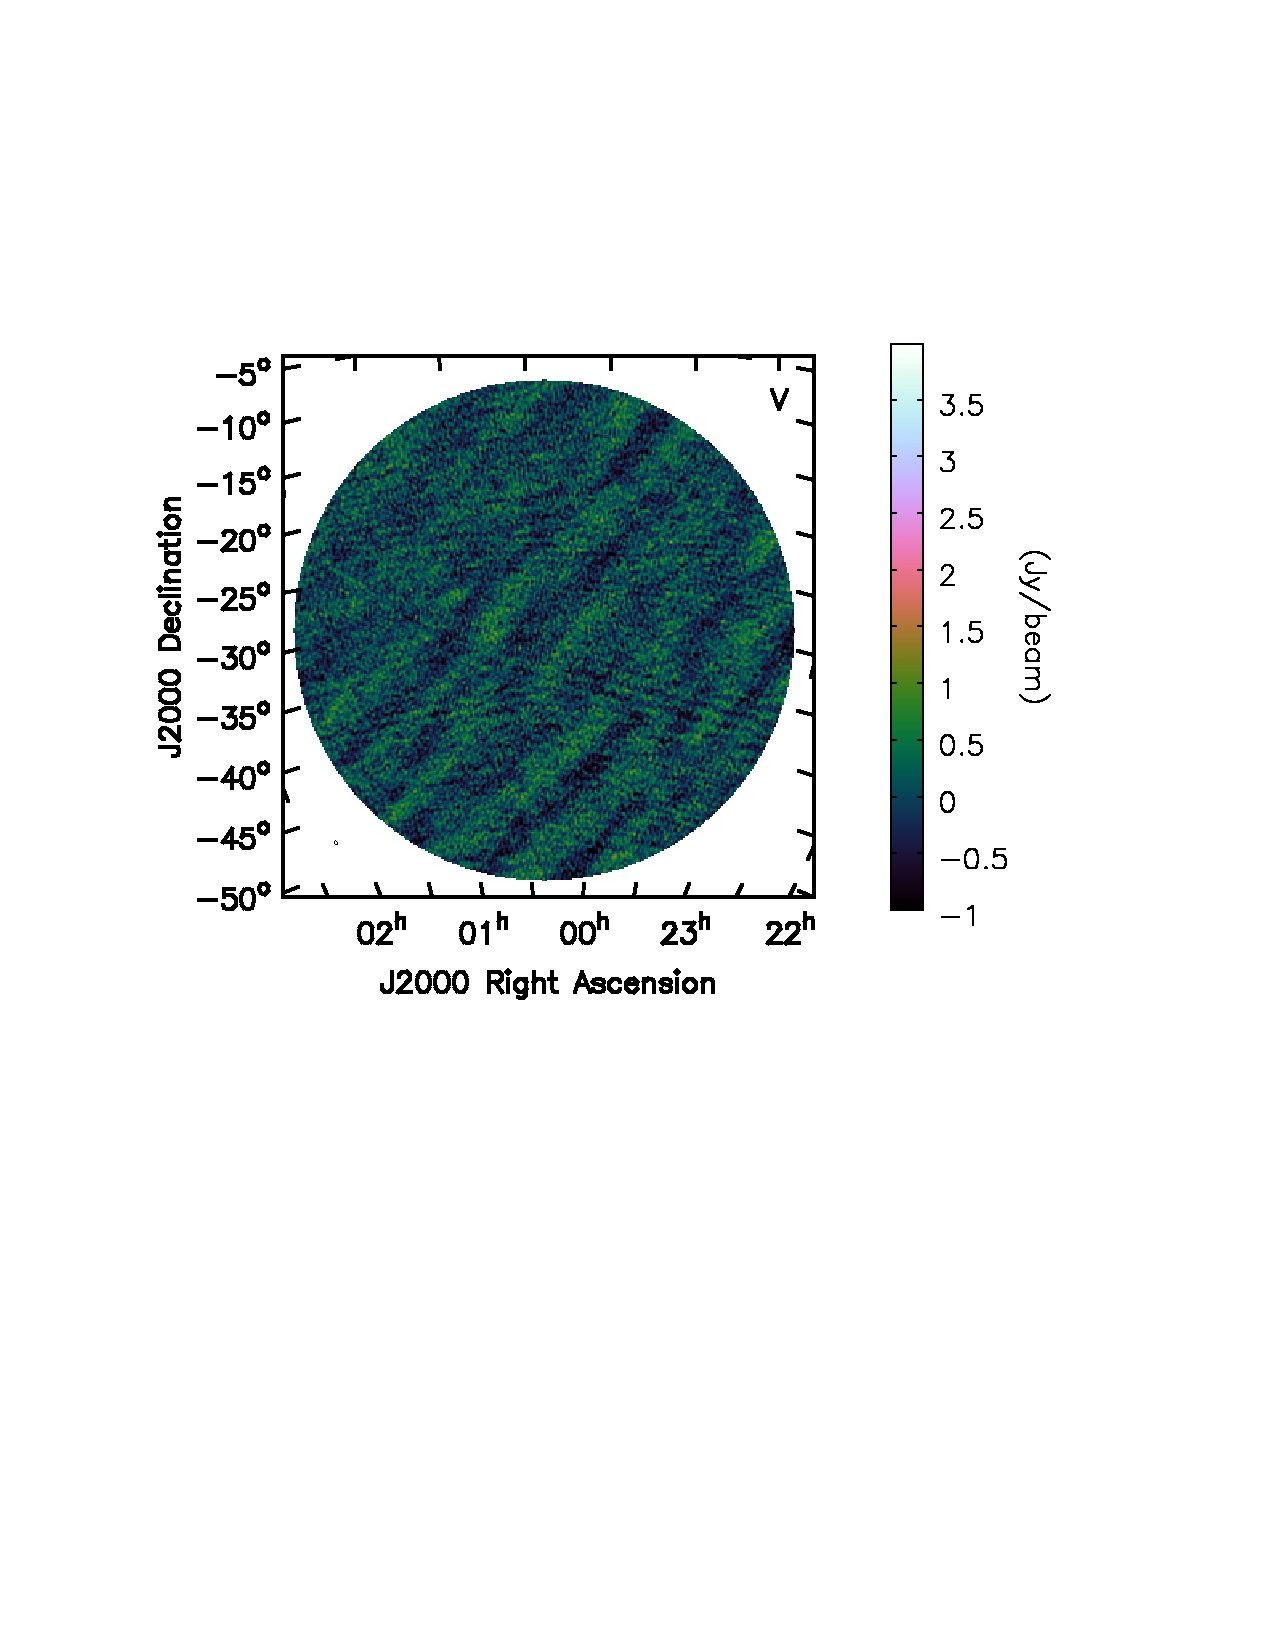
\includegraphics[clip, trim=0.5cm 11cm 3cm 5cm, width=0.6\textwidth]{chapters/polcal/figures/47501-V-better.pdf} \\
\end{tabular}
\caption[Imaging results from a file calibrated with gain values derived from the Pictor A transit, which occurred $\sim$6 hours after these data were acquired.]{Imaging results from a file calibrated with gain values derived from the Pictor A transit, which occurred $\sim$6 hours after these data were acquired. The realistic images suggest that the instrument is stable on such time scales.}
\label{fig:polcal_img_LST05}
\end{figure}

\subsection{D-term calibration}
\label{subsec:polcal_Dterms}
% basic-basic D-term stuff following CASA recipe

Calibration of the off-diagonal terms of the instrumental Jones matrix can be partially calculated using a Stokes I-only sky model. If there were a visible source of known polarization fraction, an absolute phasing could be derived based on its polarization angle. Using the source model described in the section above, we were able to calculate the magnitude of the off-diagonal, \textit{D}-terms.

{\tt CASA} supplies routines for linear-basis feeds that iteratively solve for `x' and `y' gains by, in our case, maximizing pseudo-Stokes I and minimizing pseudo-Stokes Q (if the polarization fraction was known, it would regress on that fraction for pseudo-Stokes Q). The {\tt polcal} routine uses a built-in regressor to find the best fit for the \textit{D}-terms, given previous calibrations. That is, one must have supplied an initial gain calibration and a guess of the parallactic angle of the polarized source.

Using {\tt polcal} on the Pictor A field described in the previous section granted \textit{D}-term estimates of $\sim5\%$; comparable to other low-frequency instruments (MWA-32 was found to have $\sim2$\% \textit{D}-terms [G. Bernardi, private communication]). Correcting for these granted identical pseudo-Stokes I and Q images and lower-amplitude pseudo-Stokes U and V -- as expected for a regime where pseudo-Stokes I leakage dominates over actual polarized power. The improved U and V maps are shown in Figure~\ref{fig:polcal_img_PicA_improved_dterm}.

\begin{figure}
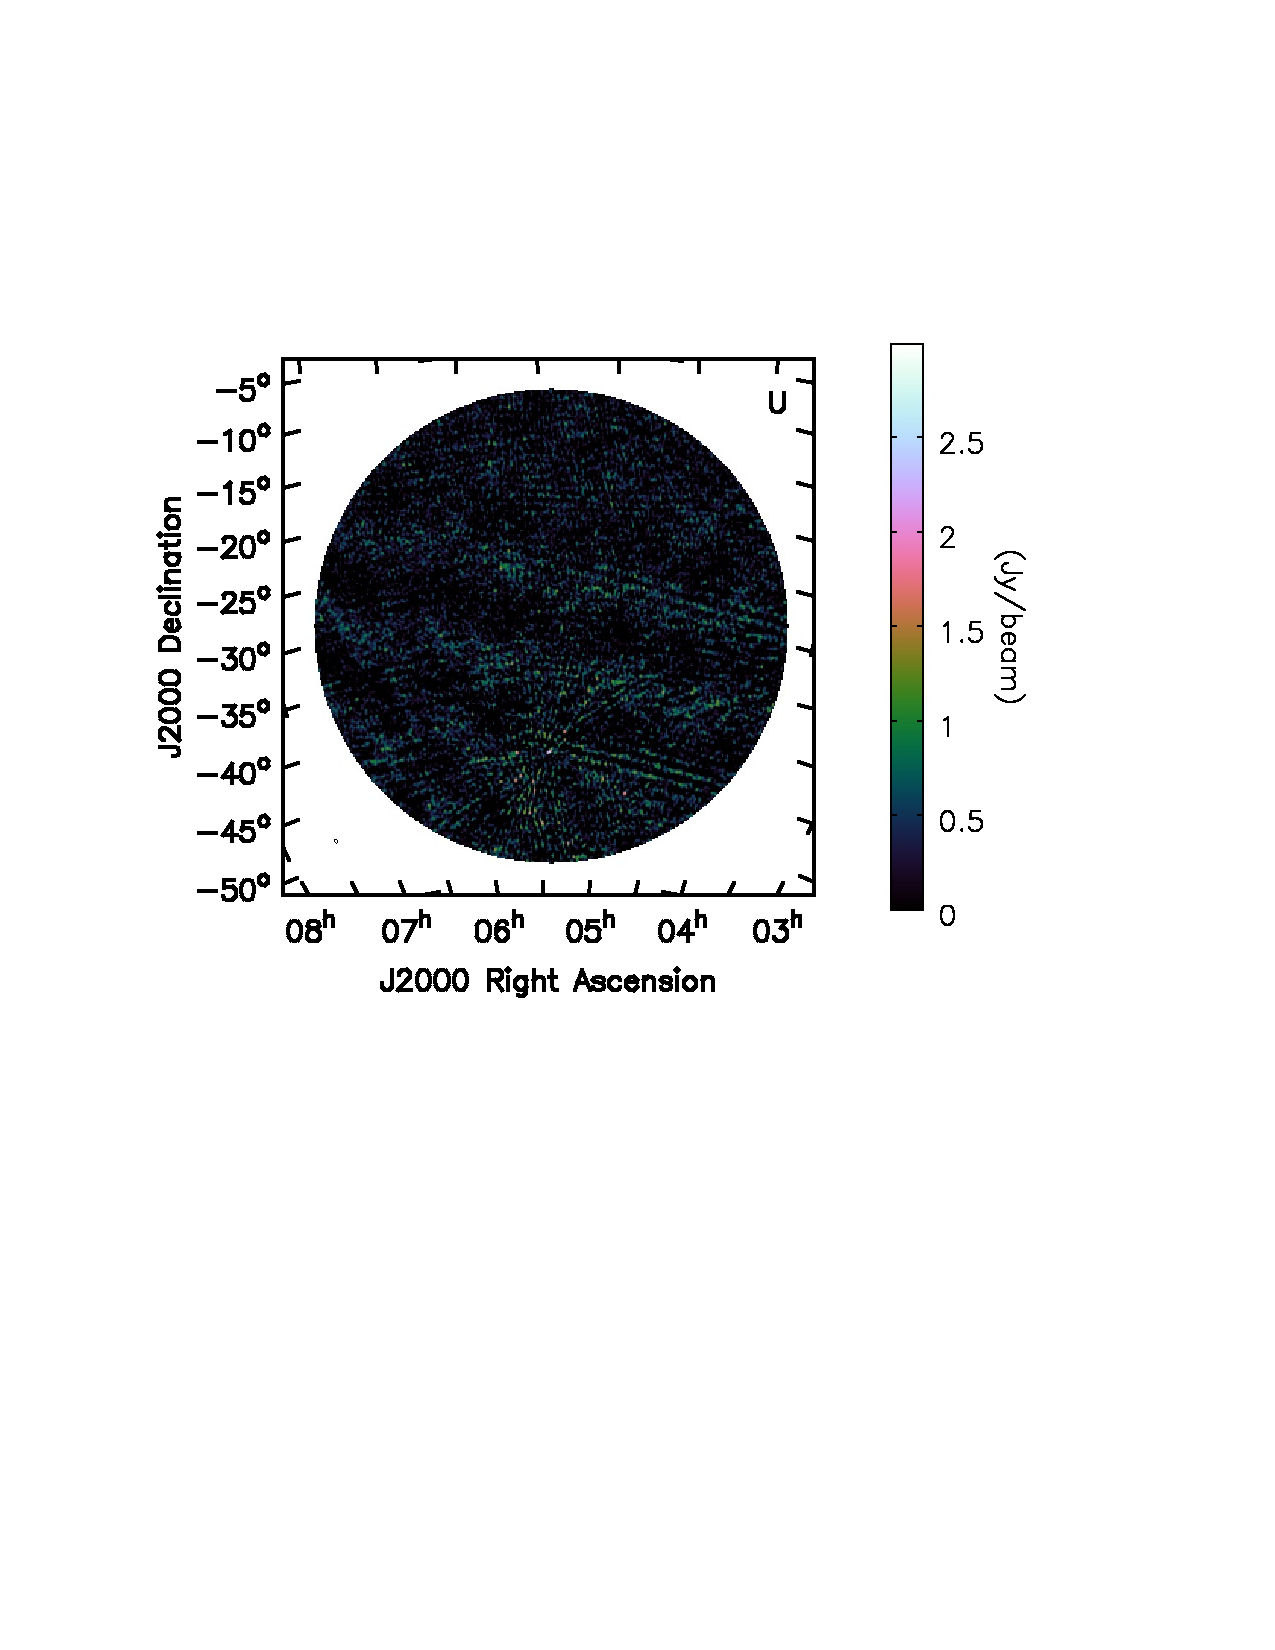
\includegraphics[clip, trim=0.5cm 11cm 4cm 5cm, width=0.8\textwidth]{chapters/polcal/figures/6830-U-better-dcal.pdf}
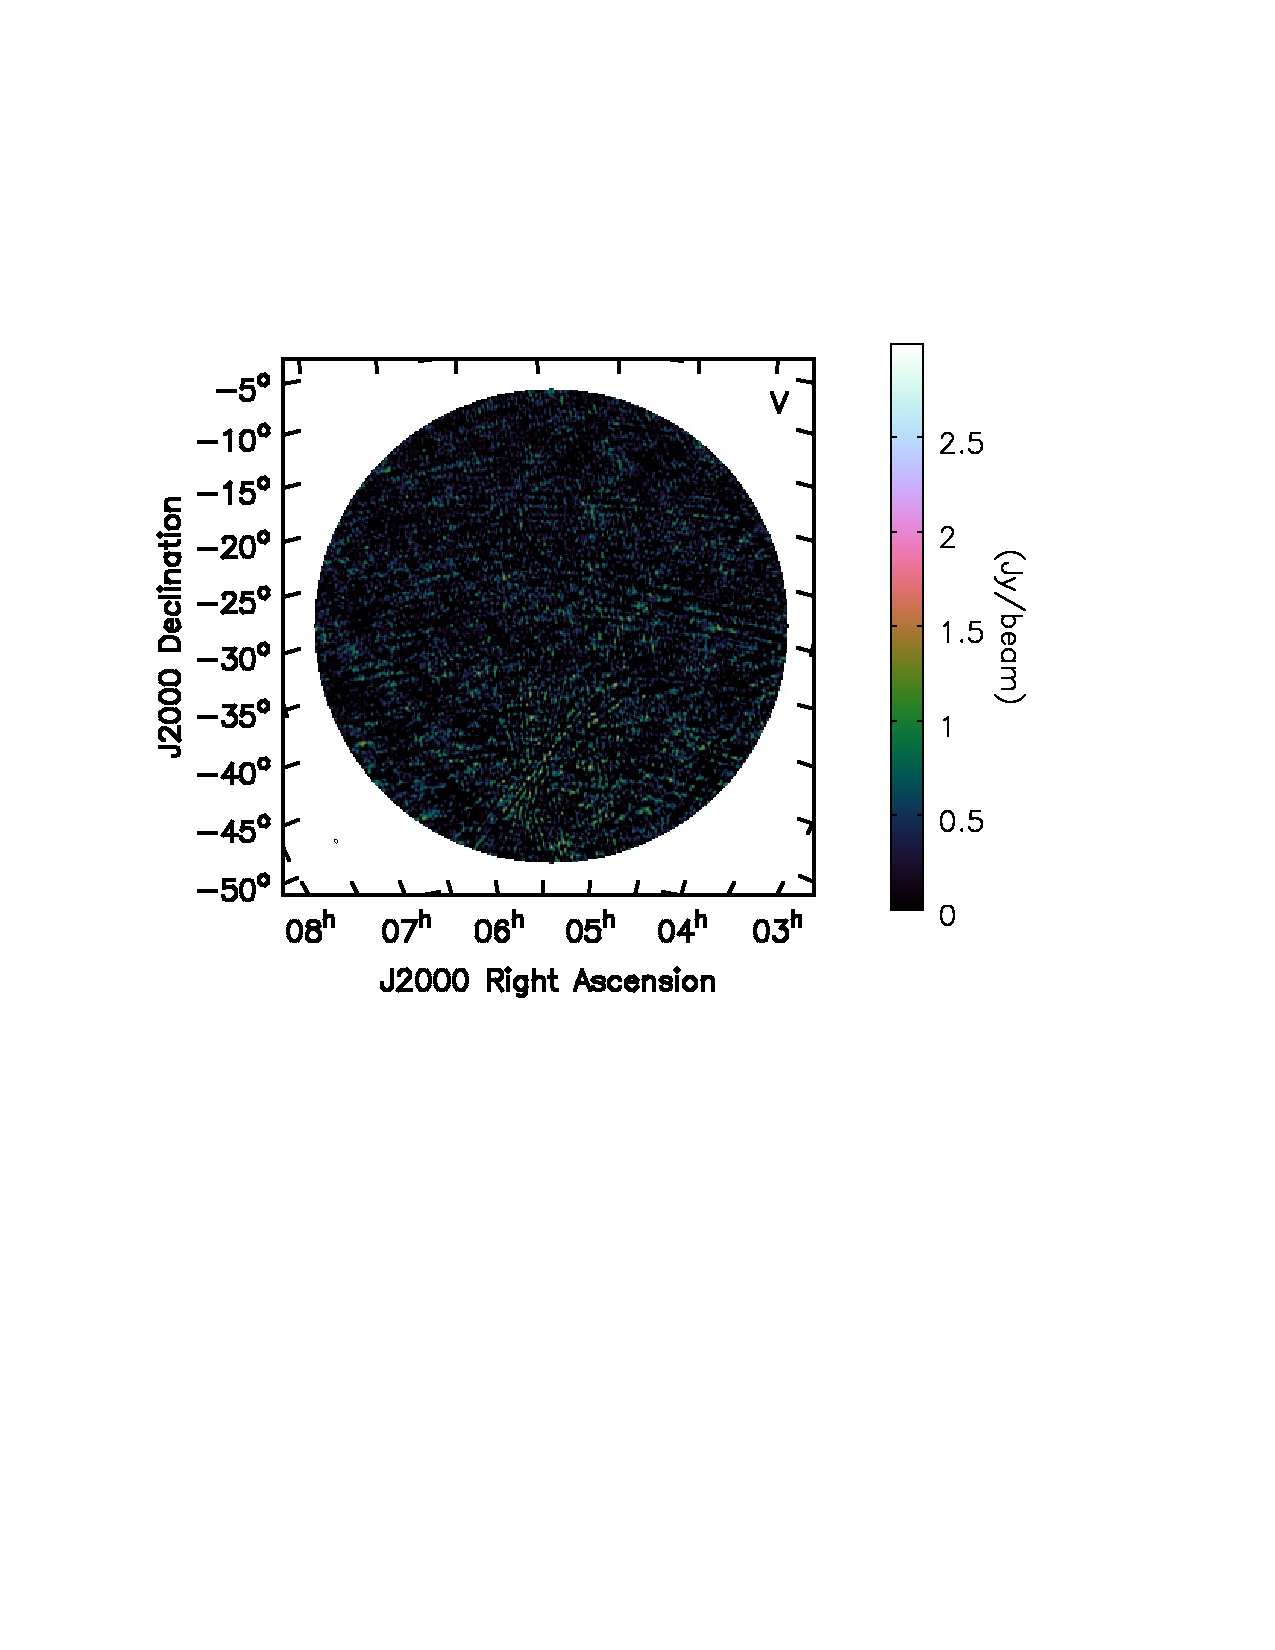
\includegraphics[clip, trim=0.5cm 11cm 4cm 5cm, width=0.8\textwidth]{chapters/polcal/figures/6830-V-better-dcal.pdf}
\caption[The same field as shown in Figure~\ref{fig:polcal_img_PicA_improved}, but for pseudo Stokes U and V only, with \textit{D}-terms partially calibrated.]{The same field as shown in Figure~\ref{fig:polcal_img_PicA_improved}, but for pseudo Stokes U and V only, with \textit{D}-terms partially calibrated. Comparing to Figure~\ref{fig:polcal_img_PicA_improved}, the amplitude at the position of Pictor A has decreased. Pseudo-Stokes I and Q maps are not shown, since they are qualitatively identical to the images in Figure~\ref{fig:polcal_img_PicA_improved} -- as expected for a regime in which pseudo-Stokes I leakage dominates over actual polarized power.}
\label{fig:polcal_img_PicA_improved_dterm}
\end{figure}



